\section{Definite integrals and Fundamental Theorem of Calculus}

In certain application scenarios, we would want to evaluate the area under the curve of a function (bounded by the $x$-axis).  For example, in economics, suppose we have supply and demand curves shown in the graph below, where $P$ stands for price, $Q$ stands for quantity, $D(Q)$ is the demand function, $S(Q)$ is the supply function, and $P^*$, $Q^*$ are the price and demand under equilibrium.  Then the \textit{consumer surplus} is defined as the shaded area marked with "CS", and the \textit{producer surplus} is defined as the shaded area marked with "PS".  It is then clear that the consumer surplus can be evaluated by subtracting $P^*Q^*$ from the area under $D(Q)$ from $Q = 0$ to $Q = Q^*$.  The producer surplus can be calculated as $P^*Q^*$ minus the area under $S(Q)$ from $Q = 0$ to $Q = Q^*$.  Therefore, it would be convenient if we could 
come up with a notation to express areas under curves and develop a technique to evaluate them.

\medskip
\begin{figure}[ht]
    \centering
    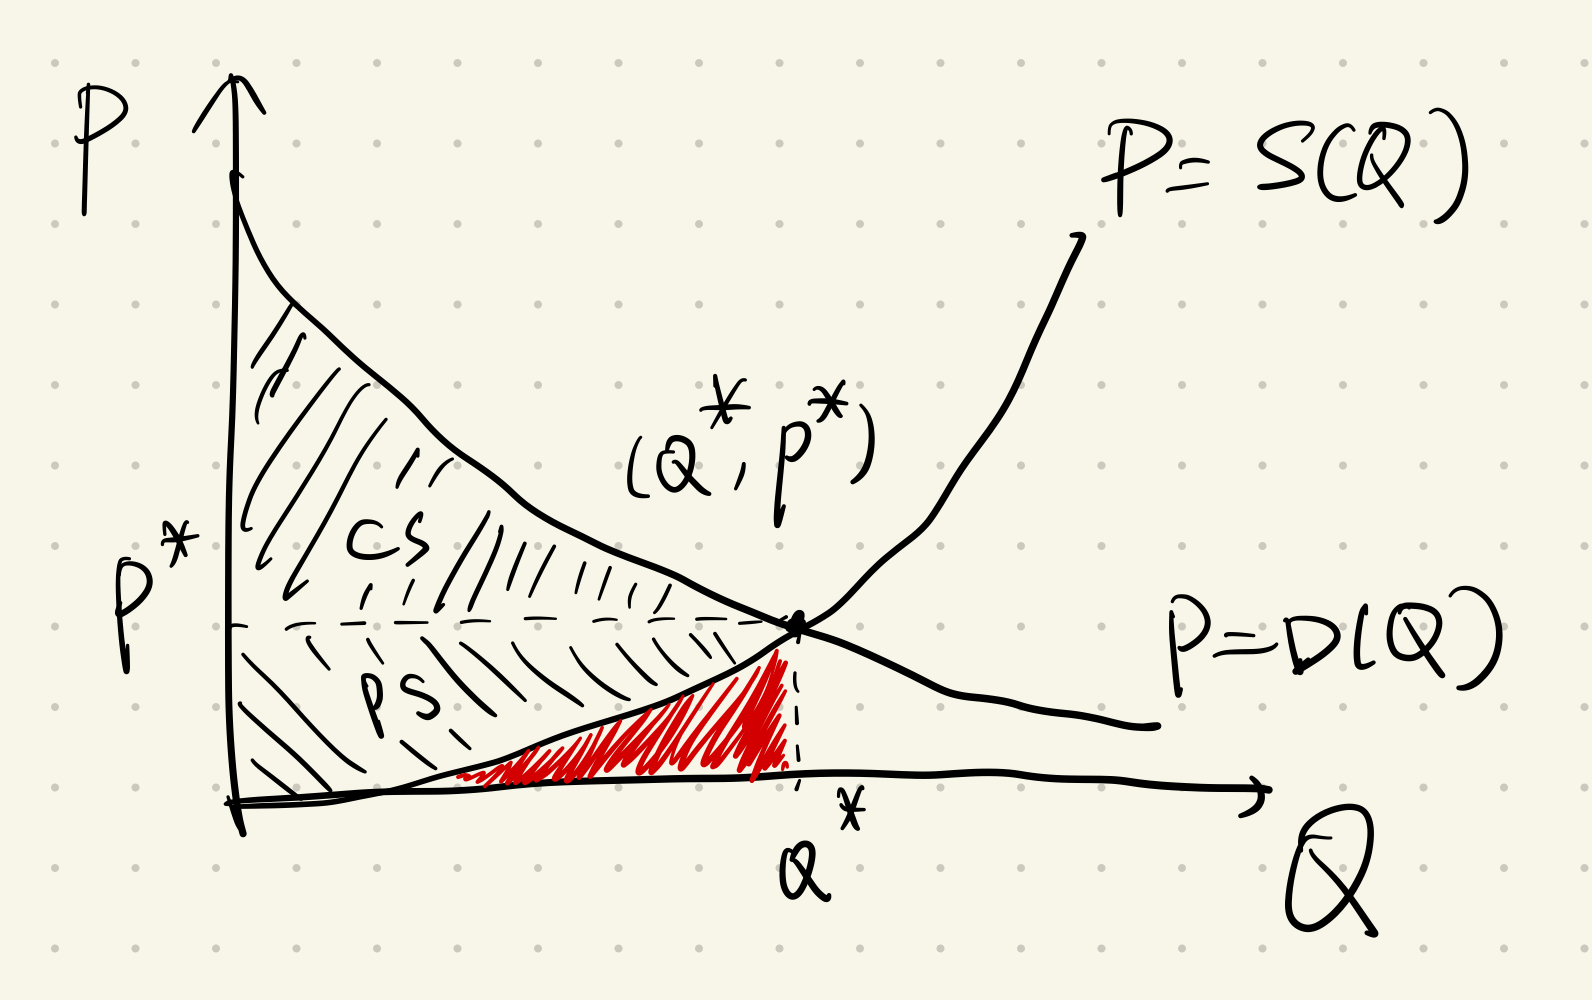
\includegraphics[width = 0.7\textwidth]{figures/chap 07/supply_demand.png}
\end{figure}

\medskip
A side note is that, in the example above, $D(Q)$ and $S(Q)$ are always positive, so it makes sense to talk about area \textit{under} the curve.  However, for functions taking negative values like the what the following graph depicts, the area bound by the curve and the $x$-axis is actually \textit{above} the curve.  In this case, for mathematical consistency, we use the notion of \textbf{signed area}, where areas above the curve and under the $x$-axis like this is given a negative sign.  With the concept of area-under-curve and signed area established, we can now define definite integrals as follows:

\begin{figure}[ht]
    \centering
    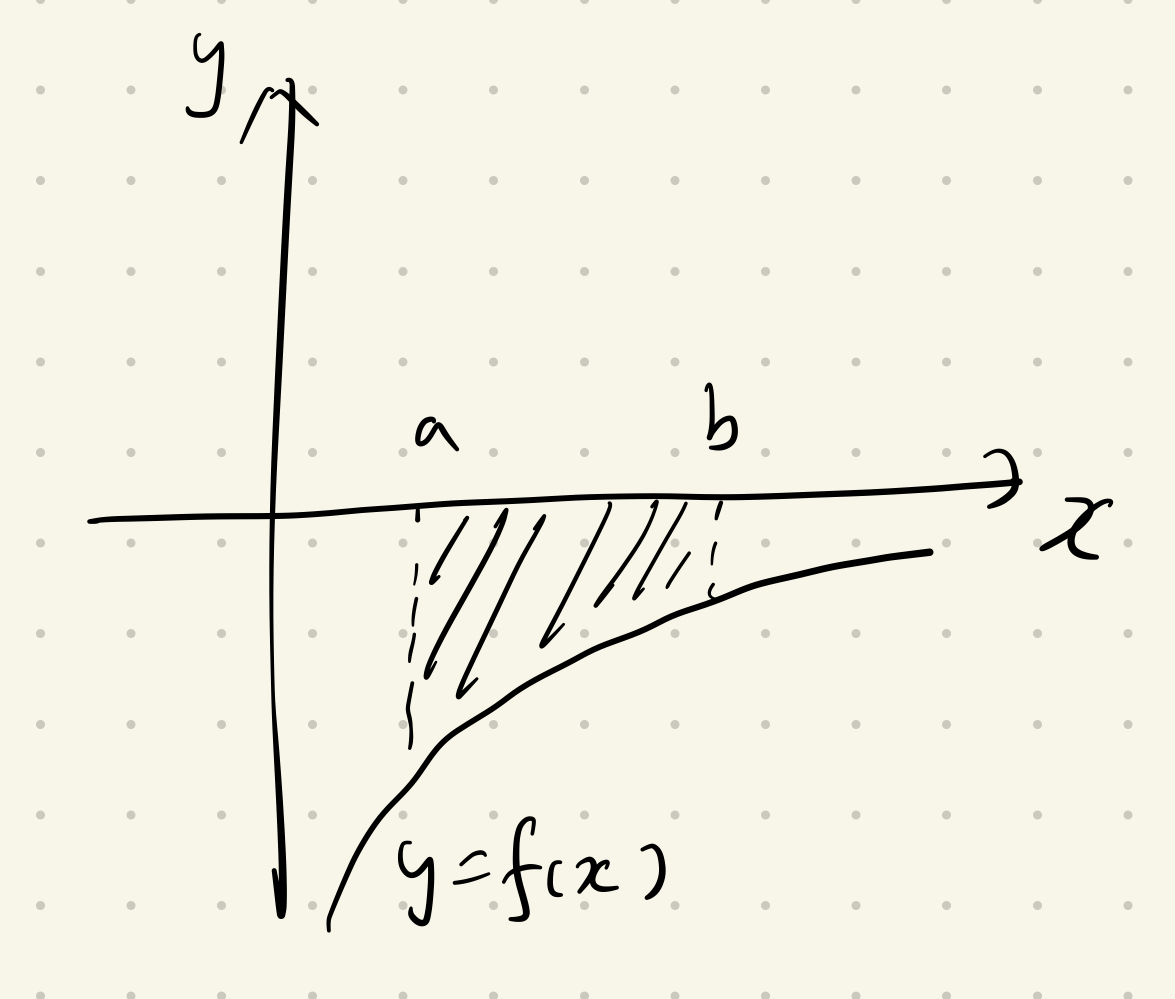
\includegraphics[width = 0.5\textwidth]{figures/chap 07/signed_area.png}
\end{figure}

\begin{defi}[Definite integrals]{def: definite_integral}
    Let $f(x)$ be a continuous function on a closed interval $[a,b]$.  The signed area bounded by the curve of $f(x)$, the $x$-axis, $x=a$ and $x=b$ is called the \textbf{definite integral} of $f(x)$ from $a$ to $b$, denoted by
    \[\int_a^b f(x)~dx\]
    where $a$ and $b$ are termed the lower and upper limit of integration for the definite integral.
\end{defi}

From this definition, if we go back to our previous example, we can notate the cosumer and producer surplus by:
\begin{align*}
    \text{Consumer surplus} &= \Big[\int_0^{Q^*} D(Q) dQ\Big] - P^*Q^*\\
    \text{Producer surplus} &= P^*Q^* - \Big[\int_0^{Q^*} S(Q) dQ\Big]
\end{align*}

Note that since definite integrals represent areas under curve, we have the following identities for definite integrals:
\begin{itemize}
    \item $\int_a^b kf(x)~dx = k\int_a^b f(x)~dx$
    \item $\int_a^b [f(x) \pm g(x)]~dx = \int_a^b f(x)~dx \pm \int_a^b g(x)~dx$
    \item $\int_a^b f(x)~dx = \int_a^c f(x)~dx + \int_c^b f(x)~dx$
    \item $\int_a^a f(x)~dx = 0$
    \item $\int_a^b f(x)~dx = -\int_b^a f(x)~dx$
\end{itemize}
where in the third identity, the area under $f(x)$ between $x = a$ and $x = b$ is intuitively decomposed into the sum of area under curve between $x = a$ and $x = c$, and area under curve between $x = c$ and $x = b$.  Setting $c = a$ in the third identity would lead to 
\[\int_a^b f(x)~dx = \int_a^a f(x)~dx + \int_a^b f(x)~dx\]
\[0 = \int_a^a f(x)~dx\]
which is exactly the fourth identity.  Setting $b = a$ in the third identity would instead lead to
\[\int_a^a f(x)~dx = \int_a^c f(x)~dx + \int_c^a f(x)~dx\]
\[\int_c^a f(x)~dx = -\int_a^c f(x)~dx \]
which implies the fifth identity: switching the upper and lower limit of a definite integral adds a negative sign to it. 

Some definite integrals can be evaluated using our knowledge in geometry.  Let's look at the following examples:

\begin{eg}[]{eg: definite_integrals}
    Using the definition of definite integrals, evaluate the following expressions:
    \begin{tasks}(3)
        \task $\int_0^2 (3x+1)~dx$
        \task $\int_2^4 (2x-5)~dx$
        \task $\int_3^1 \sqrt{4-(x-1)^2}~dx$
    \end{tasks}
\end{eg}

\begin{egsol}[]{egsol: definite_integrals}
    \begin{enumerate}[a)]
        \item If we graph $f(x) = 3x+1$ on the Cartesian plane, we see that the area under the curve from $x=0$ to $x=2$ forms a trapezoid shown in the graph below.  The two bases of the trapezoid are $f(0) = 1$ and $f(2) = 7$, and its height is $2$, so the area would be $\frac{(7+1)\cdot 2}{2} = 8$.  Therefore, the definite integral evaluates to $8$.

        \medskip
        \begin{center}
            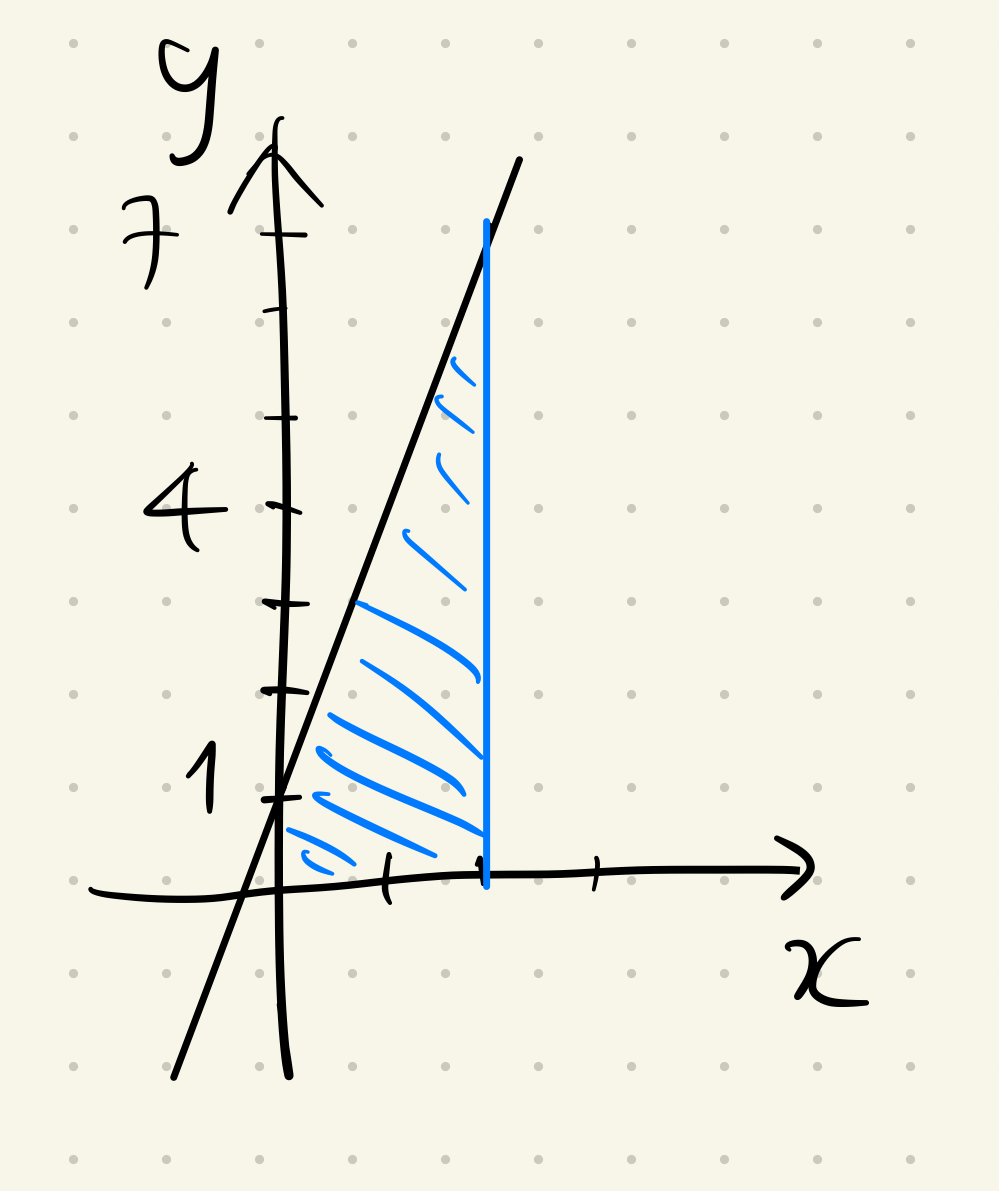
\includegraphics[width = 0.3\textwidth]{figures/chap 07/def_int_a.png}
        \end{center}
        \item If we graph $f(x) = 2x-5$ on the Cartesian plane, we see that between $x = 2$ and $x = 4$, part of the function is below the $x$-axis, and part of it is above the axis.  Since definite integrals are defined as signed area under the curves, we'll have to subtract the triangle below the axis from the triangle above the axis.  Using the identity of similar triangles, we know that since the height of the two triangles are $f(4) = 3$ and $|f(2)|=1$, their bases should be $2\cdot\frac{3}{1+3} = \frac{3}{2}$ and $2\cdot\frac{1}{1+3} = \frac{1}{2}$.  Therefore, the definite integral should evaluate to $\frac{3\cdot3/2}{2}-\frac{1\cdot1/2}{2} = 2$.
        
        \medskip
        \begin{center}
            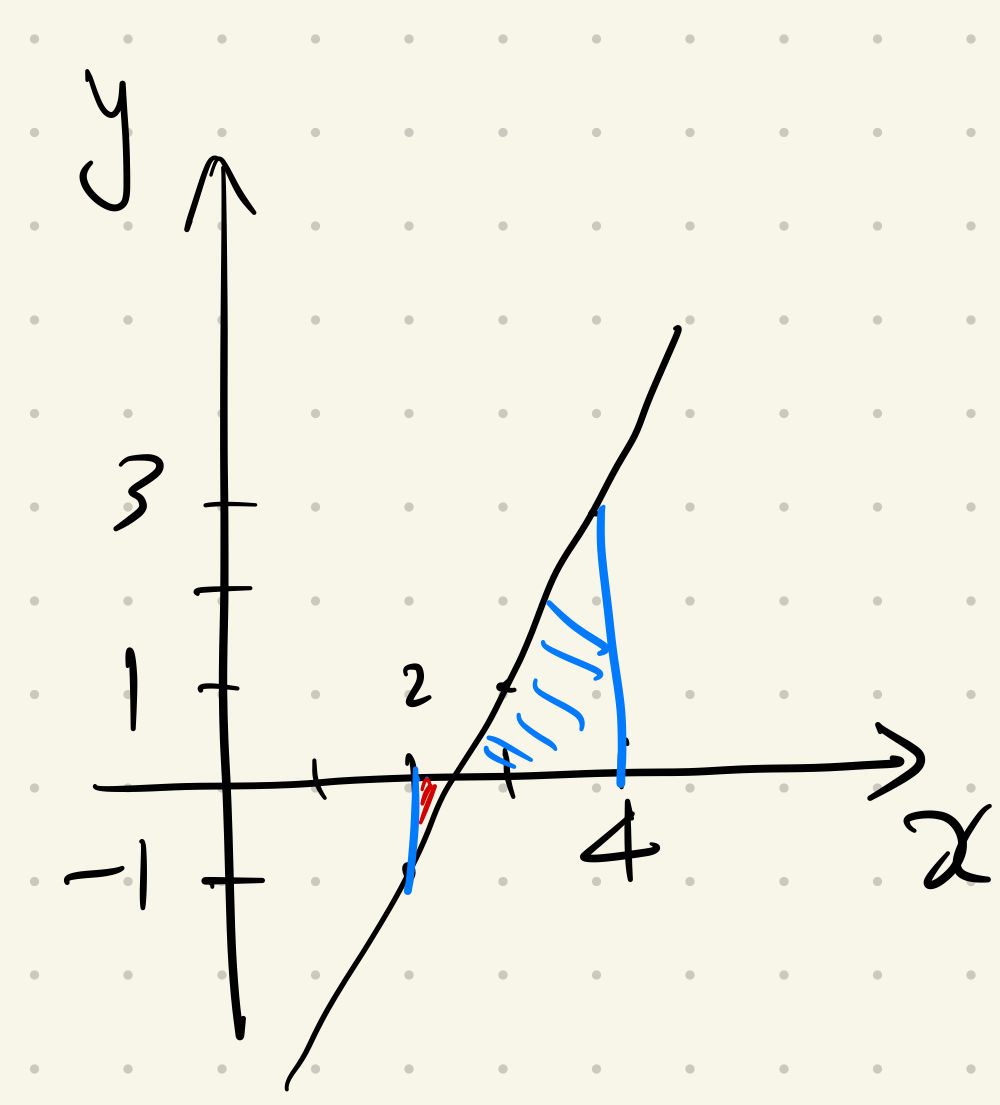
\includegraphics[width = 0.3\textwidth]{figures/chap 07/def_int_b.png}
        \end{center}
        \item Before we start graphing the function, note that upper limit of integration is smaller than its lower limit of integration, which is against our original definition.  However, using the identity we derived above, we can write
        \[\int_3^1 \sqrt{4-(x-1)^2}~dx = - \int_1^3 \sqrt{4-(x-1)^2}~dx\]
        Now the upper limit is larger than the lower limit, we can graph $f(x) = \sqrt{4 - (x-1)^2}$ on the Cartesian plane.  Rearranging $y = \sqrt{4 - (x-1)^2}$ yields $(x-1)^2 + y^2 = 2^2$, which implies that the curve of $f(x)$ is a half circle centered at $(1,0)$ with radius $2$.  Therefore, the area under the curve between $x=1$ and $x=3$ is a quarter of the circle, which has area $\pi\cdot(2)^2/4 = \pi$.  Therefore, our original definite integral evaluates to $-\pi$.
        
        \medskip
        \begin{center}
            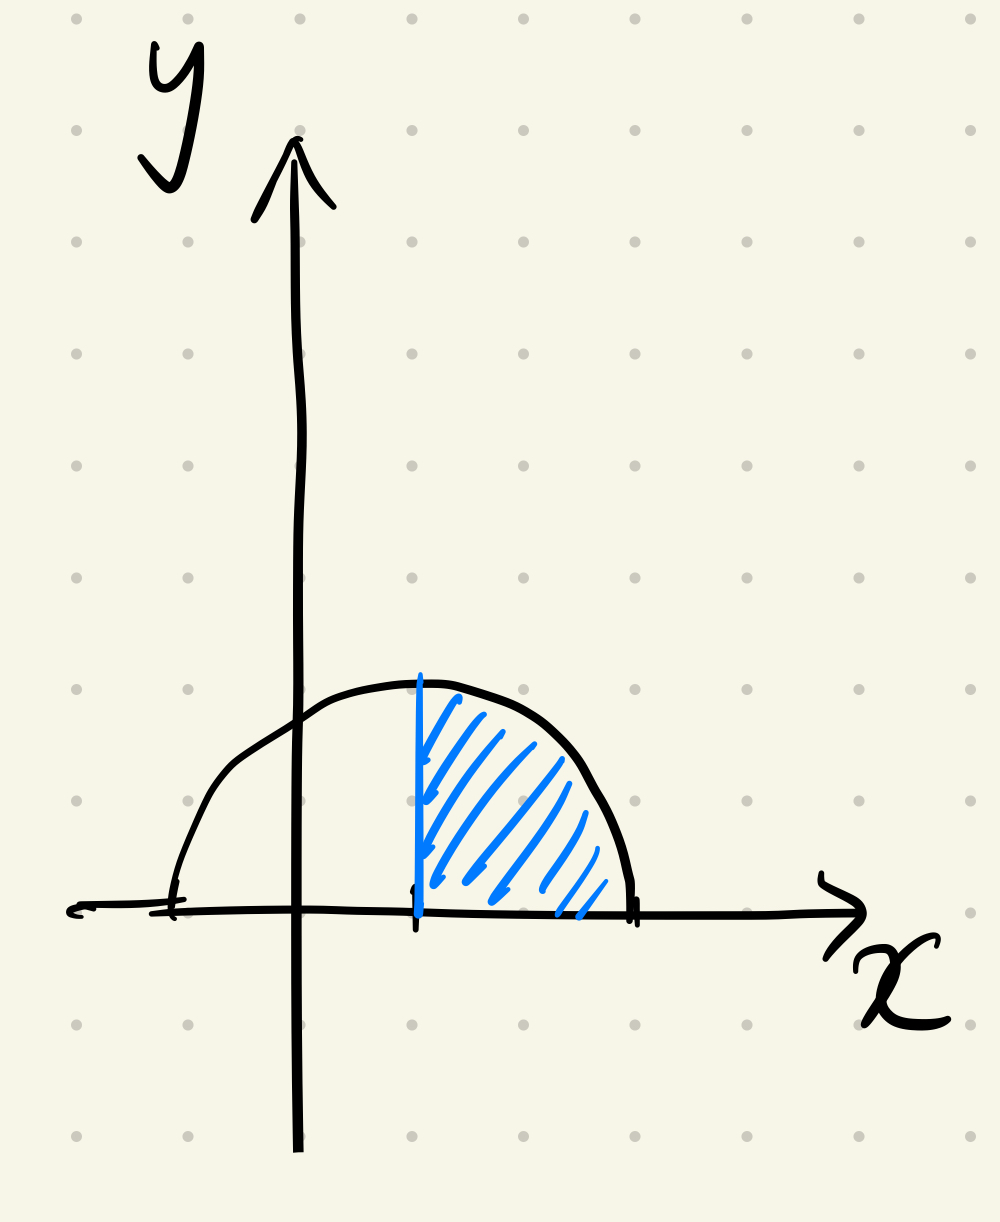
\includegraphics[width = 0.3\textwidth]{figures/chap 07/def_int_c.png}
        \end{center}
    \end{enumerate}
\end{egsol}

In the example above, the functions to be integrated represent straight lines and circles, so the area under the curves all formed shapes we are familiar with.  However, when the functions do not represent lines and circles, evaluating the integral will be much more difficult.  For example, suppose we would like to like to evaluate $\int_0^2 x^2~dx$, whose integrand is a upward-facing parabola as shown in the graph below.  One way to approach the area under curve is to first split the integration interval into smaller subintervals.  For example, in the graph, we split $[0, 2]$ into $8$ subintervals of length $\Delta x_{(8)} = 2/8$.  Then, the area under the curve can be approximated by the sum of the area of the blue bars, each with width $\Delta x_{(8)}$ and height $f(0 + j \Delta x_{(8)})$, where $j$ is the index of the subintervals ranging from $1$ to $8$.  We can write the approximation as
\begin{align*}
    \hat{A}_8 &= (f(0 + \Delta x_{(8)}) + f(0 + 2\Delta x_{(8)}) + f(0 + 3\Delta x) + ... + f(0 + 8 \Delta x_{(8)}))\Delta x_{(8)}\\
    &= \Big[\sum_{j=1}^8 f(0+j \Delta x_{(8)})\Big]\Delta x_{(8)}\\
    &= \Big[\sum_{j=1}^8 j^2 \Delta x_{(8)}^2\Big]\Delta x_{(8)}\\
    &= \Big[\sum_{j=1}^8 j^2\Big] \Delta x_{(8)}^3 =  \Big[\sum_{j=1}^8 j^2\Big] \Big(\frac{2}{8}\Big)^3 = 204 \cdot \Big(\frac{1}{4}\Big)^3 = \frac{51}{16}
\end{align*}

\begin{figure}[ht]
    \centering
    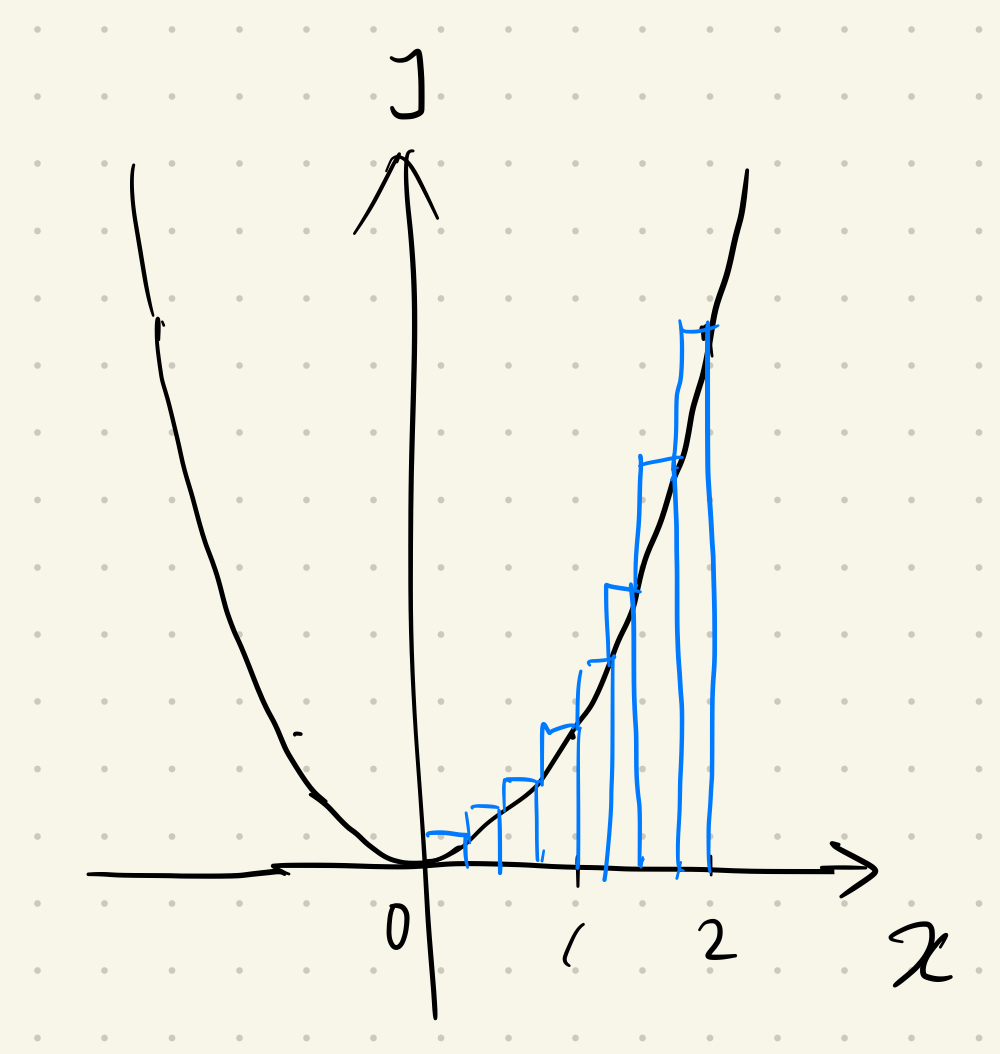
\includegraphics[width = 0.45\textwidth]{figures/chap 07/def_int_series.png}
\end{figure}

This approximation is called a (right) Riemann sum.  If we notate the number of subintervals as $n$ so that the length of the subintervals is $\Delta x_{(n)} = 2/n$, we yield a generalized Riemann sum:
\[\hat{A}_n = \Big[\sum_{j=1}^n j^2\Big] \Delta x_{(n)}^3 = \frac{n(n+1)(2n+1)}{6} \Big(\frac{2}{n}\Big)^3 = \frac{4n(n+1)(2n+1)}{3n^3}\]
where the second equality uses the formula for sum of squares of the first $n$ positive numbers.  Note as $n$ increases, the bars will be finer and finer, and the sum of the bars will eventually approach to the area under the curve.  Therefore, we can write our definite integral as a limit with $n$ approaching infinity:
\[\int_0^2 x^2~dx = \lim_{n \rightarrow \infty} \hat{A}_n = \lim_{n \rightarrow \infty} \frac{4n(n+1)(2n+1)}{3n^3} = \frac{8}{3}\]
where the last equality comes from the ratio of leading coefficients.

Here, we used the limit of Riemann sums to evaluate the definite integral, which is not an easy feat.  However, our success is not without luck: because our integrand is $x^2$, the sum of squares of the first $n$ positive numbers appeared in the Riemann sum, which we happened to know a clean formula for the sum.  If our integrand was something gnarlier, then it may well be the case that we do not have a closed form expression for the Riemann sum, and thus cannot take its limit.  In light of this, we will need a more general procedure to evaluate definite integrals. 

To develop the procedure, first we define an \textbf{area function} as a definite integral that leaves its upper limit as input.  For example, in the graph below, we define the area function $F(x) = \int_0^x f(t)~dt$, where the lower limit of integration is fixed at $0$ but the upper limit of integration is the variable $x$.  The signed area $F(x)$ represents is then by definition the area shaded blue.  

\begin{figure}[ht]
    \centering
    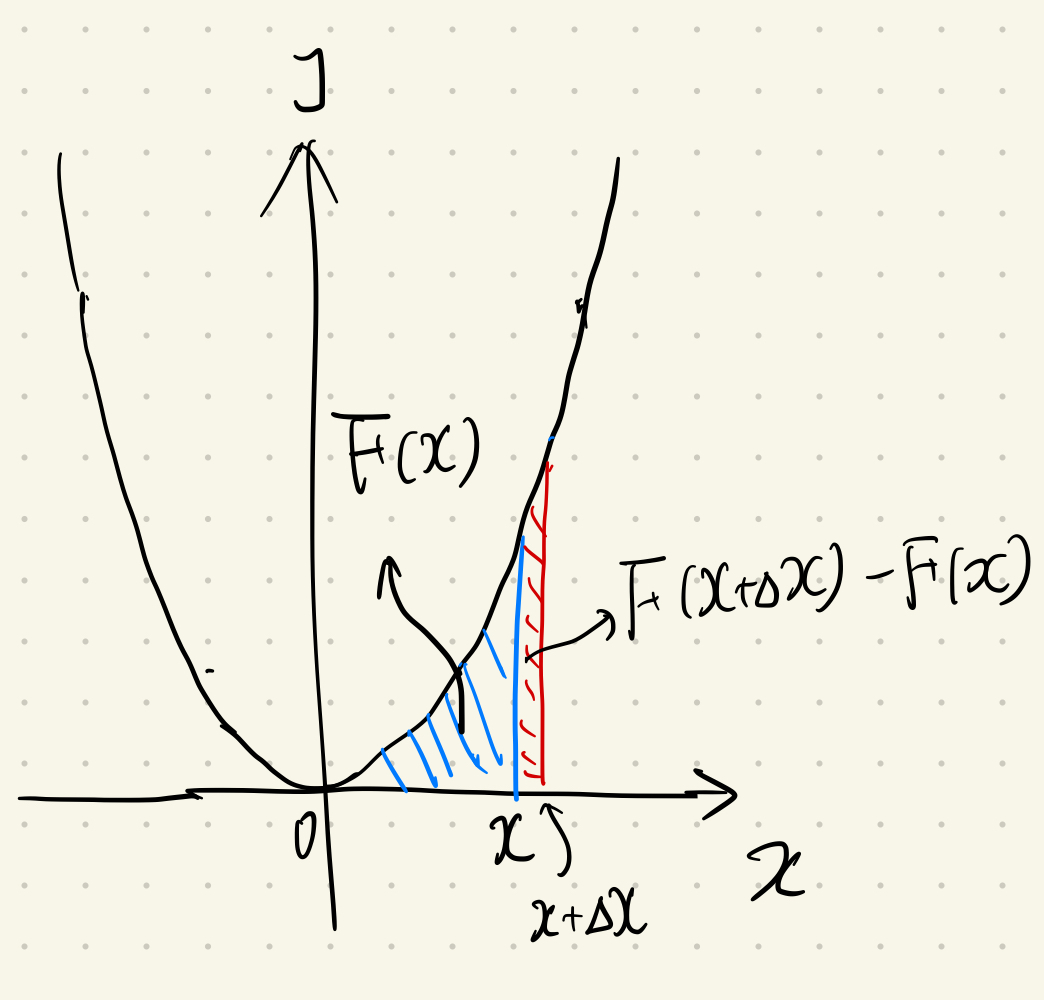
\includegraphics[width = 0.45\textwidth]{figures/chap 07/FTC.png}
\end{figure}

Now for a small $\Delta x$, the difference between $F(x+\Delta x)$ and F(x) would be the small strip of area under curve from $x$ to $x + \Delta x$, which is the area shaded red in the graph.  As $\Delta x$ gets smaller and smaller, the area of the strip would be closer and closer to $f(x) \Delta x$.  In other words, as $\Delta x$ gets smaller and smaller, the ratio between $F(x + \Delta x) - F(x)$ and $\Delta x$ would approach $f(x)$.  Therefore, we have

\[\frac{dF}{dx} = \lim_{\Delta x \rightarrow 0} \frac{F(x + \Delta x) - F(x)}{\Delta x} = f(x)\]

which implies that $F(x)$, which we originally defined as an area function, is actually an antiderivative of $f(x)$!  This remarkable result serves as a bridge between integral calculus (definite integrals) to differential calculus (antiderivatives), which we formally state in the theorem below:

\begin{theo}[Fundamental Theorem of Calculus, First Part]{thm: FTC1}
    Let $f(x)$ be a continuous function on $[a, b]$. Suppose $F(x)$ is an area function defined as 
    \[F(x) = \int_a^x f(t) dt, \quad x \in (a,b)\]
    then $F'(x) = f(x)$ for all $x \in (a,b)$.
\end{theo}

However, note that the first part of the Fundamental Theorem of Calculus only tells us that the area function $F(x)$ is \textit{an} antiderivative of $f(x)$, but does not tell us \textit{which} antiderivative it is.  That is, it does not explicitly tell us what the integration constant should be when we have obtained our antiderivative.  Fortunately, the second part of the Fundamental Theorem of Calculus tells us that as long as we are only interested in evaluating the definite integral, the choice of integration constant does not matter (it also relaxes the requirement for $f(x)$ to be continuous, but here we will not dig deeper into this issue):

\medskip
\begin{theo}[Fundamental Theorem of Calculus, Second Part]{thm: FTC2}
    Let $f(x)$ be a function on $[a, b]$.  Let $F(x)$ be \textit{any} antiderivative for $f(x)$, then
    \[\int_a^b f(x) dx = F(b) - F(a)\]
\end{theo}

Therefore, to find the definite integral for $f(x)$ from $a$ to $b$, we just need to find \textit{one} antiderivative for $f(x)$, and subtract its value at $x = b$ by its value at $x = a$.  Here since antiderivatives are closely linked to the evaluation of definite integrals, they are alternatively termed as \textbf{indefinite integrals}.

Let us try out our new evaluation method for definite integrals with a few examples:

\begin{eg}[]{eg: def_int_FTC}
    Evaluate the following definite integrals
    \begin{tasks}(3)
        \task $\int_0^2 x^2~dx$
        \task $\int_{\pi/2}^{0} \sin x~dx$
        \task $\int_1^{\sqrt{3}} \frac{1}{x^2+1}~dx$
        \task $\int_0^1 \frac{x}{x^2+1}~dx$
        \task $\int_{1/2}^{\sqrt{3}/2} \frac{1}{(\sqrt{1-x^2})^3}~dx$
        \task $\int_{0}^{\pi/4} x \cos x~dx$
    \end{tasks}
\end{eg}

\begin{egsol}[]{egsol: def_int_FTC}
    \begin{enumerate}[a)]
        \item We have evaluated this definite integral the hard way using Riemann sums.  Now let us try using antiderivatives and the Fundamental Theorem of Calculus.  Since one antiderivative of $x^2$ is $\frac{1}{3}x^3$, we can write:
        \[\int_0^2 x^2~dx = \frac{1}{3}x^3\Big]^2_0 = \frac{1}{3}(2)^3 - \frac{1}{3}(0)^3 = \frac{8}{3}\]
        where the notation $g(x)\big]^b_a$ stands for $g(b)-g(a)$.  Antiderivatives have indeed saved us much time here.
        \item Since one antiderivative of $\sin x$ is $-\cos x$, we have
        \[\int_{\pi/2}^0 \sin x~dx = (-\cos x)\Big]_{\pi/2}^0 = -\cos(0) + \cos(\pi/2) = -1 + 0 = -1\]
        Note here we do not even care if the upper limit of integration is larger than the lower limit.  We can just evaluate our antiderivatives with the correct order of subtraction, and the Fundamental Theorem of Calculus will take care of the rest.
        \item Remember that one antiderivative of $\frac{1}{x^2+1}$ is $\arctan x$, so we have
        \[\int_1^{\sqrt{3}} \frac{1}{x^2+1}~dx = \arctan x\Big]_1^{\sqrt{3}} = \arctan(\sqrt{3}) - \arctan(1) = \frac{\pi}{3} - \frac{\pi}{4} = \frac{\pi}{12}\]
        \item The antiderivative for this integrand is not immediately obvious, but if we try U-substituion with $u = x^2+1$, we have $du = 2xdx$, which works since the remainder of the integrand is $x$.  Therefore, we have
        \[\int_0^1 \frac{x}{x^2+1} dx = \frac{1}{2}\int_0^1 \frac{1}{x^2+1}(2xdx)\]
        Now note that when we preform variable substitutions in definite integrals, we will also have to substitute the limits of integration.  That is, originally we are integrating from $x = 0$ to $x = 1$, but now we are changing our variable for integration to $u$, the limits of integration should then be from $u = 0^2+1 = 1$ to $u = 1^2 + 1 = 2$.  We then yield
        \[\frac{1}{2}\int_0^1 \frac{1}{x^2+1}(2xdx) = \frac{1}{2} \int_1^2 \frac{1}{u} du = \frac{1}{2}(\ln |u|)\Big]_1^2 = \frac{1}{2}(\ln |2| - \ln |1|) = \frac{\ln 2}{2}\]
        \item The $\sqrt{1-x^2}$ in the denominator screams for a trigonometric substitution where $x = \sin \theta$ and $dx = \cos \theta d\theta$, but note that since we are performing variable substitution, we need to also transform the limits of integration.  This is where the range setting for $\theta$ becomes important.  Since we by convention set $-\pi/2 \le \theta \le \pi/2$, we have when $x = 1/2$ and $\sqrt{3}/2$, $\theta = \pi/6$ and $\pi/3$. Therefore we yield
        \begin{align*}
            \int_{1/2}^{\sqrt{3}/2} \frac{1}{(\sqrt{1-x^2})^3}~dx &= \int_{\pi/6}^{\pi/3} \frac{1}{\cos^3 \theta}\cos \theta d\theta\\
            &= \int_{\pi/6}^{\pi/3} \sec^2 \theta d\theta\\
            &= \tan \theta \Big]_{\pi/6}^{\pi/3}\\
            &= \tan\Big(\frac{\pi}{3}\Big) - \tan\Big(\frac{\pi}{3}\Big) = \sqrt{3} - \frac{1}{\sqrt{3}} = \frac{2}{3}\sqrt{3}
        \end{align*}
        \item Here the antiderivative can be found using integration by parts setting $u = x$ and $dv/dx = \cos x$, so that $du/dx = 1$ and $v = \sin x$.  Therefore we have
        \begin{align*}
            \int_{0}^{\pi/4} x \cos x~dx &= x \sin x \Big]_{0}^{\pi/4} - \int_{0}^{\pi/4} \sin x~dx\\
            &= x \sin x \Big]_{0}^{\pi/4} + \int_{0}^{\pi/4} (-\sin x)~dx\\
            &= x \sin x \Big]_{0}^{\pi/4} + \cos x \Big]_{0}^{\pi/4}\\
            &= \Big(\frac{\pi}{4} \sin \frac{\pi}{4} - 0 \sin 0\Big) + \Big(\cos \frac{\pi}{4} - \cos 0 \Big)\\
            &= \frac{\pi}{4} \cdot \frac{\sqrt{2}}{2} + \frac{\sqrt{2}}{2} - 1 = \frac{\sqrt{2}}{8}\pi + \frac{\sqrt{2}}{2}- 1
        \end{align*}
        Note that since this is a definite integral, the "$uv$" term is also subject to calculation of value difference at limits of integration, so don't forget to put a right bracket beside it!
    \end{enumerate}
\end{egsol}

\section{Area and arc length}

In the previous section we defined definite integrals as the area under the curve of a function, and showed that definite integrals can be promptly evaluated using antiderivatives.  However, definite integrals can do much more than calculating the area under the curve.  

To extend the use of definite integrals, first recall that back when we did not know how to use antiderivatives to evaluate definite integrals, we turned to the limit of Riemann sums, which can be written and graphed as follows 
\[\int_a^b f(x) dx = \lim_{\Delta x \rightarrow 0} \sum_{i=1}^n f(x_i) \Delta x\]
\begin{figure}[ht]
    \centering
    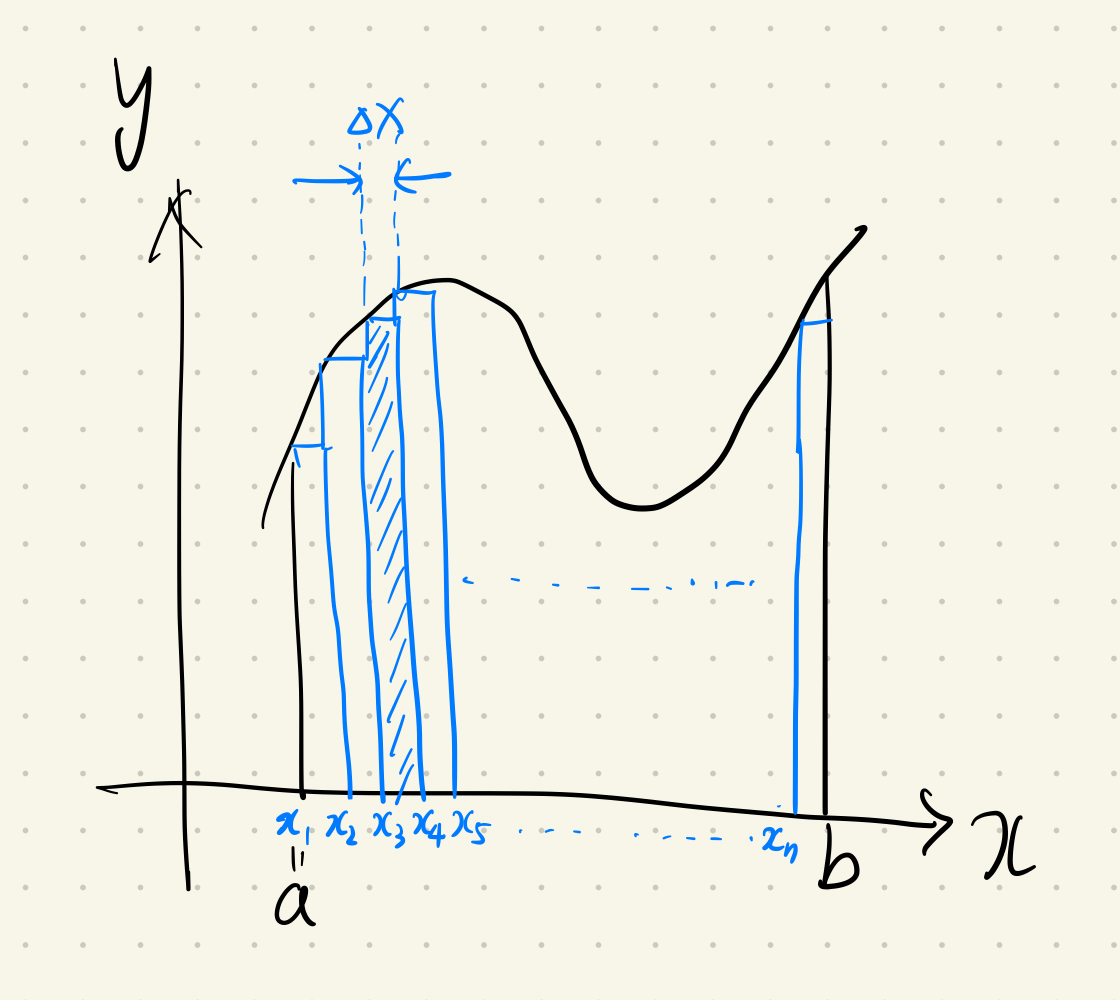
\includegraphics[width = 0.5\textwidth]{figures/chap 07/Riemann.png}
\end{figure}

\bigskip
In the right hand side, the term $f(x_i) \Delta x$ is the area of the strip of rectangle at $x = x_i$ with width $\Delta x$.  For example, $f(x_3)\Delta x$ represents the area of the blue strip shown in the graph.  Then, the summation sign adds all the strips up, with the $x$-coordinates of the strip ranging from $a$ to $b$.  Roughly speaking, as $\Delta x$ goes to zero, $f(x_i)\Delta x$ can be replaced with $f(x)dx$, and the summation sign can be replaced with $\int_a^b$, which re-frames the limit of summation into limit of integration.  The limit of integration specifies the limit of the variable indicated by the differential, which in this case is $x$.

With this correspondence in mind, we do not have to resort to writing out the limit of Riemann sums everytime we want to find a definite integral.  Instead, as shown in the left panel below, we can directly say that the area under $y = f(x)$ between $x = a$ and $x = b$ is just adding up the area of small shaded strips while $x$ goes from $a$ to $b$.  Since the area of the small strips is $f(x)dx$, we write the area as $\int_a^b f(x)dx$. 

\begin{figure}[ht]
    \centering
    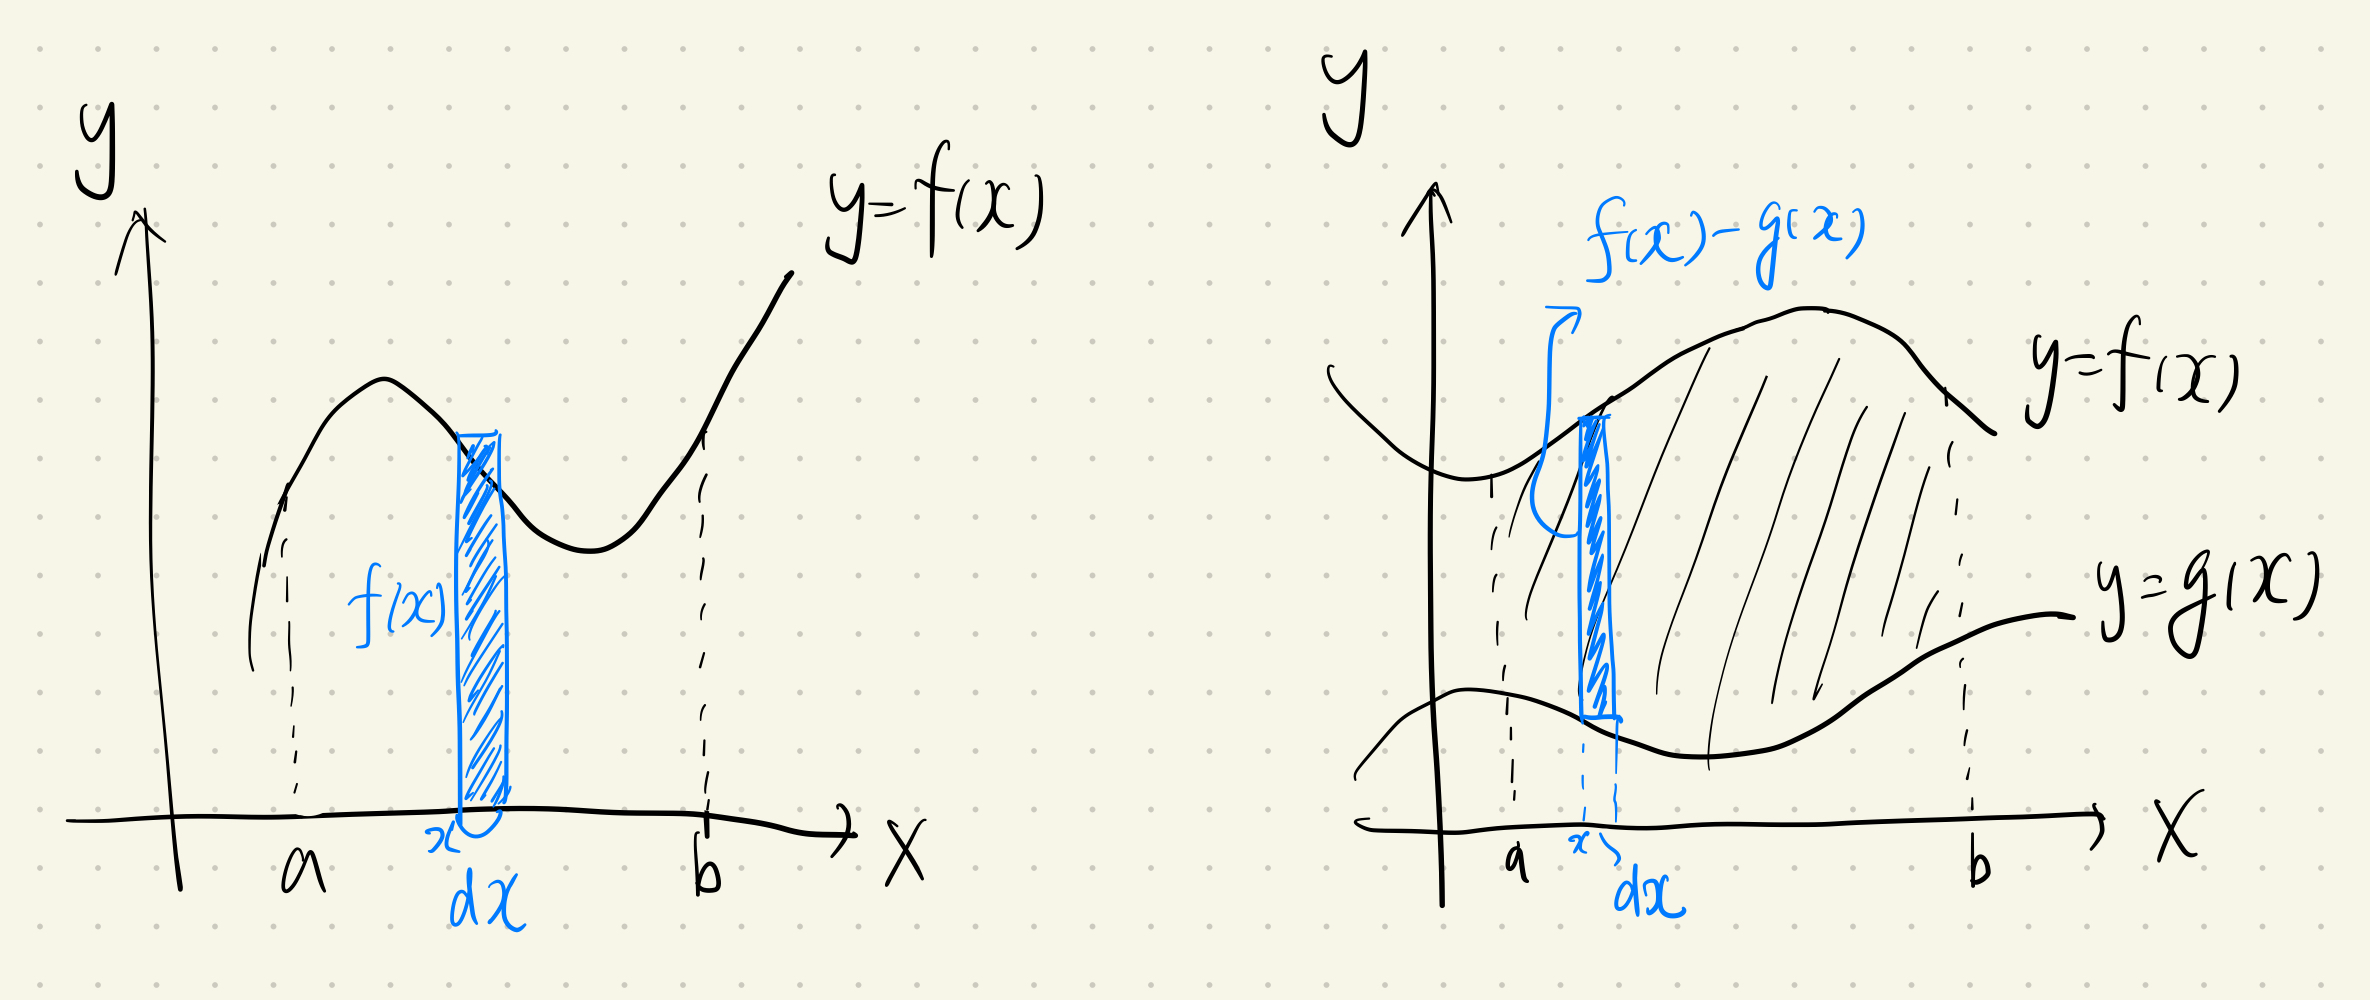
\includegraphics[width = 0.8\textwidth]{figures/chap 07/Differential_Riemann.png}
\end{figure}

This method of constructing definite integrals can be extended to the evaluation of area between the curves of two functions.  As shown in the right panel of the graph above, suppose $f(x) \ge g(x)$ within $x \in [a,b]$, and we would like to find the area enclosed by $y = f(x)$, $y = g(x)$, $x=a$ and $x=b$.  We note that the area can broken up into the sum of small shaded strips as shown in the graph, with width $dx$ and height $|f(x)-g(x)| = f(x) - g(x)$, so that the area is $(f(x)-g(x))dx$.  Since the summation ranges from $x=a$ to $x=b$, our area of interest can be written as
\[A = \int_a^b (f(x)-g(x))dx\]
Notice that in this case we are assuming that $f(x) \ge g(x)$ within $[a, b]$.  If $f(x)$ is less than $g(x)$ in any interval within $[a,b]$, then the height of the strip within that interval would be $g(x)-f(x)$, so the integrand would become $g(x)-f(x)$.  In this case, we will have to evaluate the definite integral into different parts are evaluate them separately.  We will now demonstrate its application with several examples:

\begin{eg}[]{eg: area_between_functions}
    Find the following areas using definite integrals:
    \begin{enumerate}[a)]
        \item The area between $y = (x-1)^2 + 3$ and $y = -(x-2)^2$ from $x = 1$ to $x = 3$.
        \item The area enclosed by $y = \sqrt{x}$ and $y = x^2$
        \item The area enclosed by $y = \sin x$ and $y = \cos x$ between $x = \pi/4$ to $x = 5\pi/4$
        \item The area between $y = 2x$ and $y = x^3$ from $x = -1$ to $x = 1$
    \end{enumerate}
\end{eg}

\begin{egsol}[]{egsol: area_between_functions}
    \begin{enumerate}[a)]
        \item We first graph $y = (x-1)^2 +3$ and $y = -(x-2)^2$ as follows, which shows that $(x-1)^2 +3$ is always greater than $-(x-2)^2$ between $x = 1$ and $x = 3$.  Therefore, we can directly construct the definite integral as
        \begin{align*}
            &\int_1^3 [((x-1)^2 + 3) - (-(x-2)^2)]dx\\
            =& \int_1^3 [(x^2-2x+4)+(x^2-4x+4)]dx\\
            =& \int_1^3 (2x^2-6x+8) dx\\
            =& \Big(\frac{2}{3}x^3 - 3x^2 + 8x \Big)\Big]_1^3\\
            =& \Big(\frac{2}{3}\cdot 27 - 3 \cdot 9 + 8 \cdot 3 \Big) - \Big(\frac{2}{3} - 3 + 8 \Big)\\
            =& 15 - \frac{17}{3} = \frac{28}{3} 
        \end{align*}
        \begin{center}
            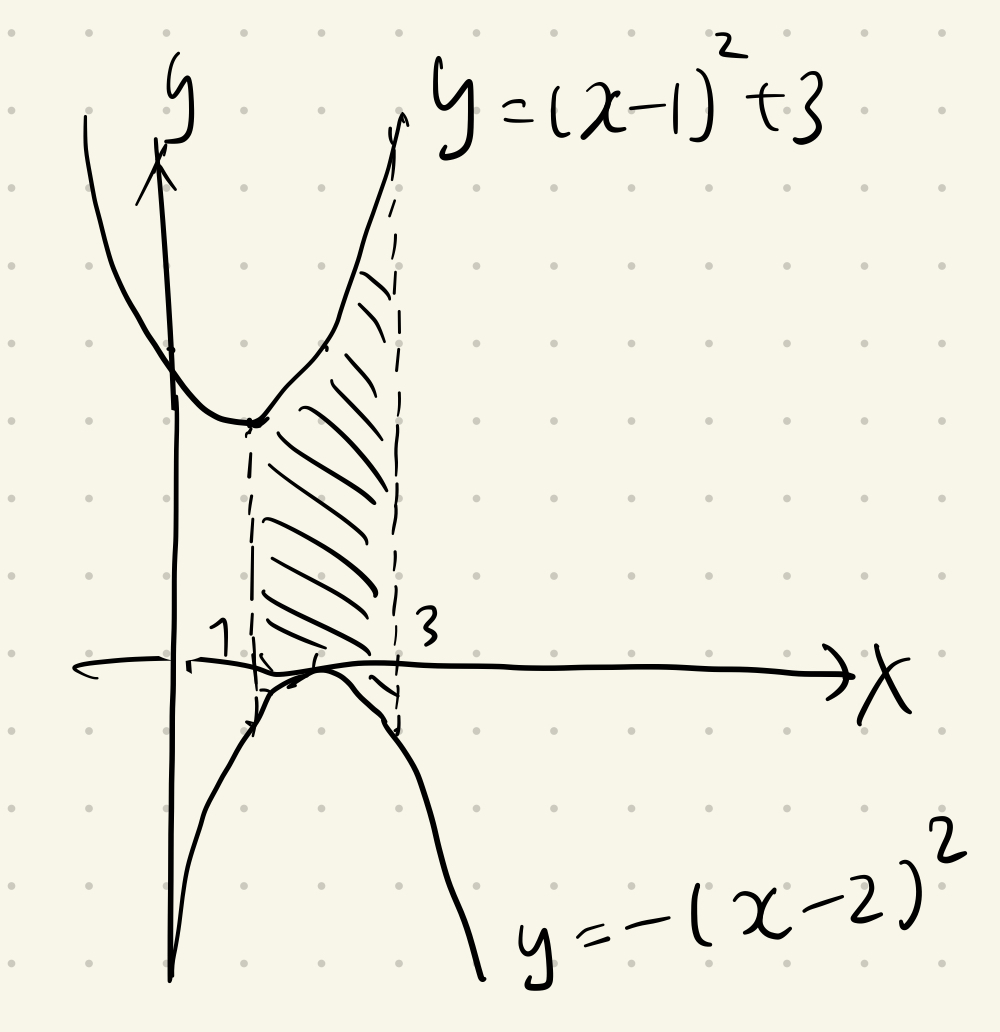
\includegraphics[width = 0.35\textwidth]{figures/chap 07/eg_7_3_a.png}
        \end{center}
        \item The problem did not give us the range of $x$ for the area enclosed by the two functions, so we first graph $y = x^2$ and $y = \sqrt{x}$.  As the following graph shows, they intersect at $(0,0)$ and $(1,1)$, and the enclosed area lies between these two points.  In addition, $\sqrt{x}$ is always no less than $x^2$ with in $x \in [0,1]$.  Therefore, we can directly construct the definite integral as
        \[\int_0^1(\sqrt{x} - x^2)~dx = \int_0^1(x^{1/2} - x^2)~dx = \Big(\frac{2}{3}x^{3/2} - \frac{1}{3}x^3\Big)\Big]_0^1 = \frac{2}{3} - \frac{1}{3} = \frac{1}{3}\]
        \begin{center}
            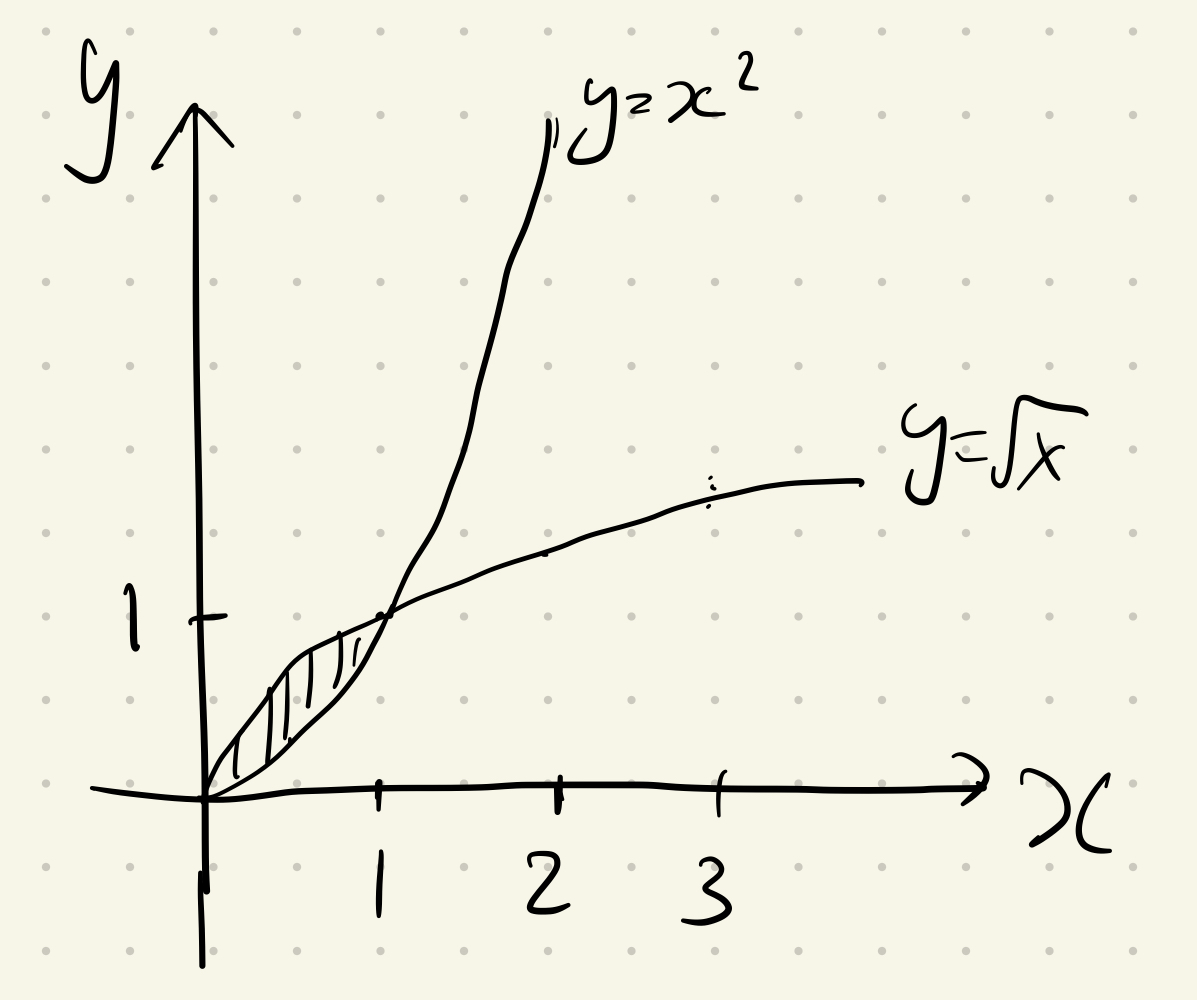
\includegraphics[width = 0.35\textwidth]{figures/chap 07/eg_7_3_b.png}
        \end{center}
        \item We first graph $y = \sin x$ and $y = \cos x$ within $x \in [\pi/4, 5\pi/4]$.  Notice that within $[\pi/4, 5\pi/4]$, we have $\sin x \ge \cos x$.  Therefore, we can directly construct the definite integral as
        \[\int_{\pi/4}^{5\pi/4} (\sin x - \cos x)~dx = (- \cos x - \sin x) \Big]_{\pi/4}^{5\pi/4} = \Big(\frac{1}{\sqrt{2}} + \frac{1}{\sqrt{2}}\Big)-\Big(-\frac{1}{\sqrt{2}} - \frac{1}{\sqrt{2}}\Big) = \frac{4}{\sqrt{2}} = 2\sqrt{2}\]
        \begin{center}
            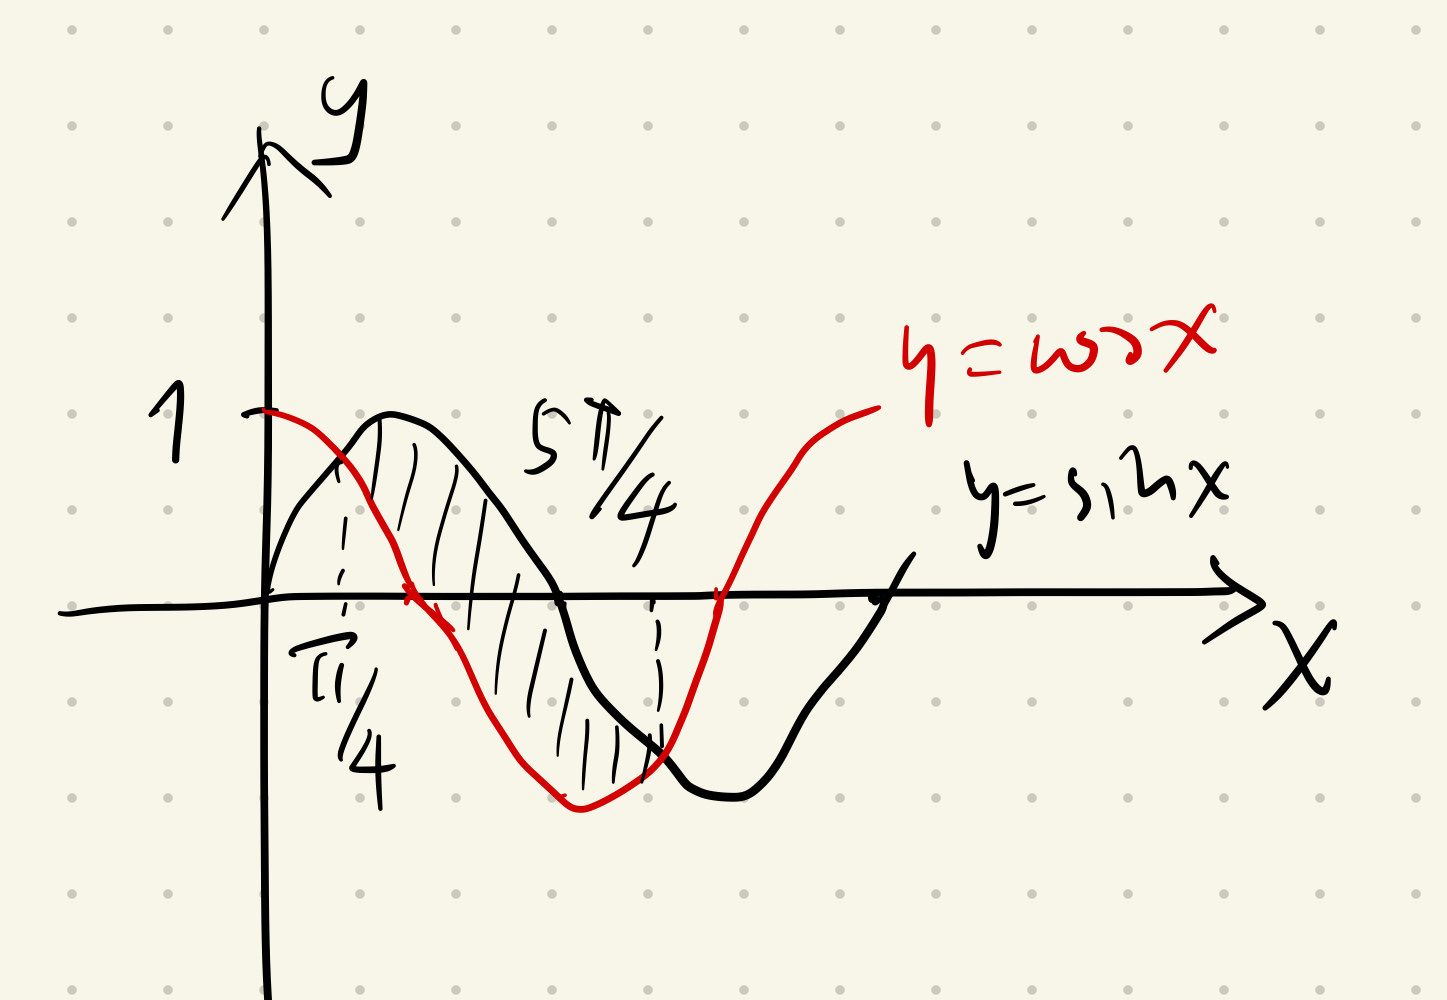
\includegraphics[width = 0.35\textwidth]{figures/chap 07/eg_7_3_c.png}
        \end{center}
        \item We first graph $y = 2x$ and $y = x^3$ within $x \in [-1, 1]$ as the follow graph, and notice that $2x > x^3$ when $x > 0$, but $x^3 > 2x$ when $x < 0$.  Therefore, we will have to construct the definite integral by splitting the range of integration into two parts, $[-1, 0]$ and $[0,1]$:
        \begin{align*}
            &\int_{-1}^0 (x^3-2x)~dx + \int_0^1 (2x-x^3)~dx\\
            =& \Big(\frac{1}{4}x^4 - x^2\Big)\Big]_{-1}^0 + \Big(x^2 - \frac{1}{4}x^4\Big)\Big]_0^1\\
            =& \Big[(0 - 0) - \Big(\frac{1}{4}-1\Big)\Big] + \Big[\Big(1 - \frac{1}{4}\Big)-(0-0)\Big] = \frac{3}{2}
        \end{align*}
        \begin{center}
            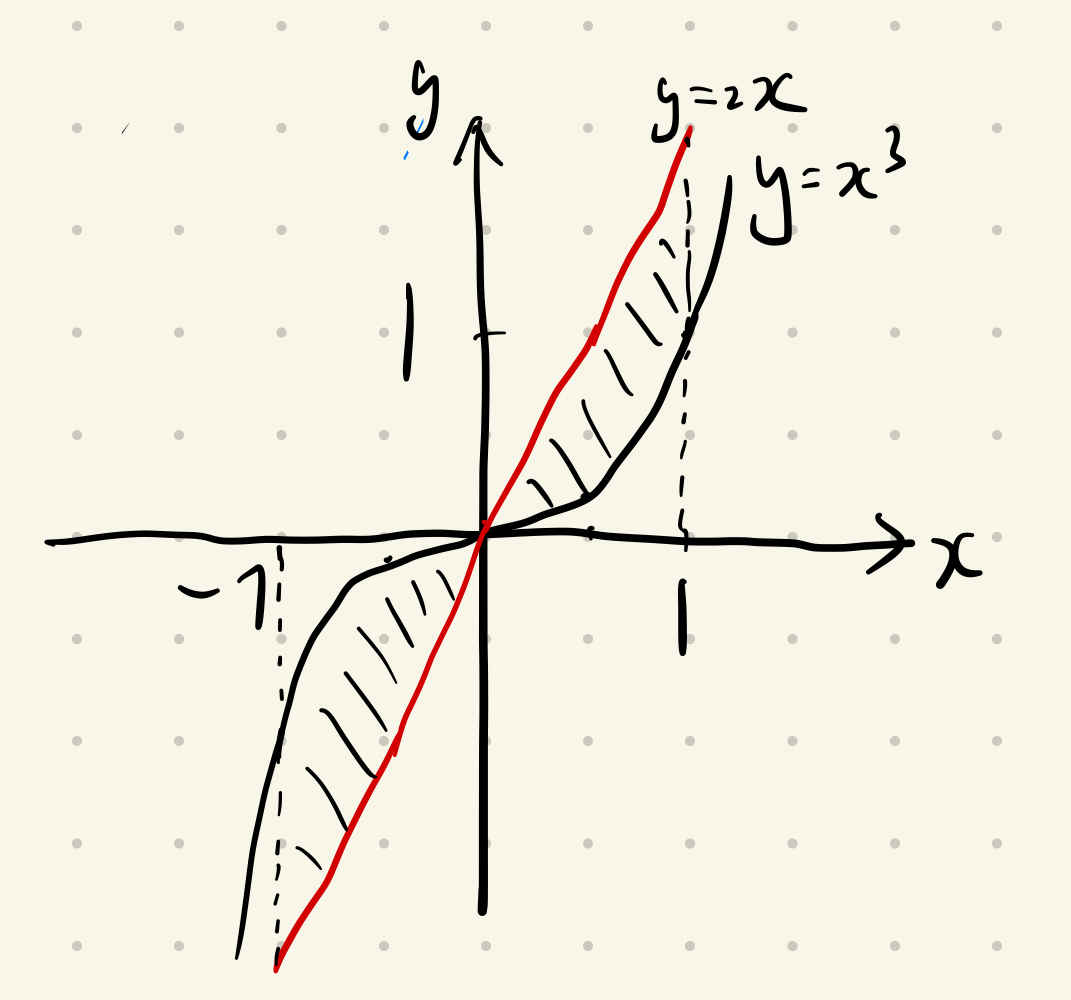
\includegraphics[width = 0.35\textwidth]{figures/chap 07/eg_7_3_d.png}
        \end{center}
        Notice that if we did not determine the order of $2x$ and $x^3$ first, and just evaluated $\int_{-1}^1 (x^3-2x)~dx$ or $\int_{-1}^1 (2x - x^3)~dx$, we would get an answer of $0$, which is clearly incorrect.
    \end{enumerate}
\end{egsol}

Apart from evaluation of areas, definite integrals can also help us find the arc length of a function, i.e. the length of its curve between two points on the curve.  To see this, lets suppose $f(x)$ is a continuous function within $x \in [a, b]$, and we wish to find the arc length of $y = f(x)$ between $(a,f(b))$ and $(b, f(b))$.  Then, we can produce the following graph:

\begin{figure}[ht]
    \centering
    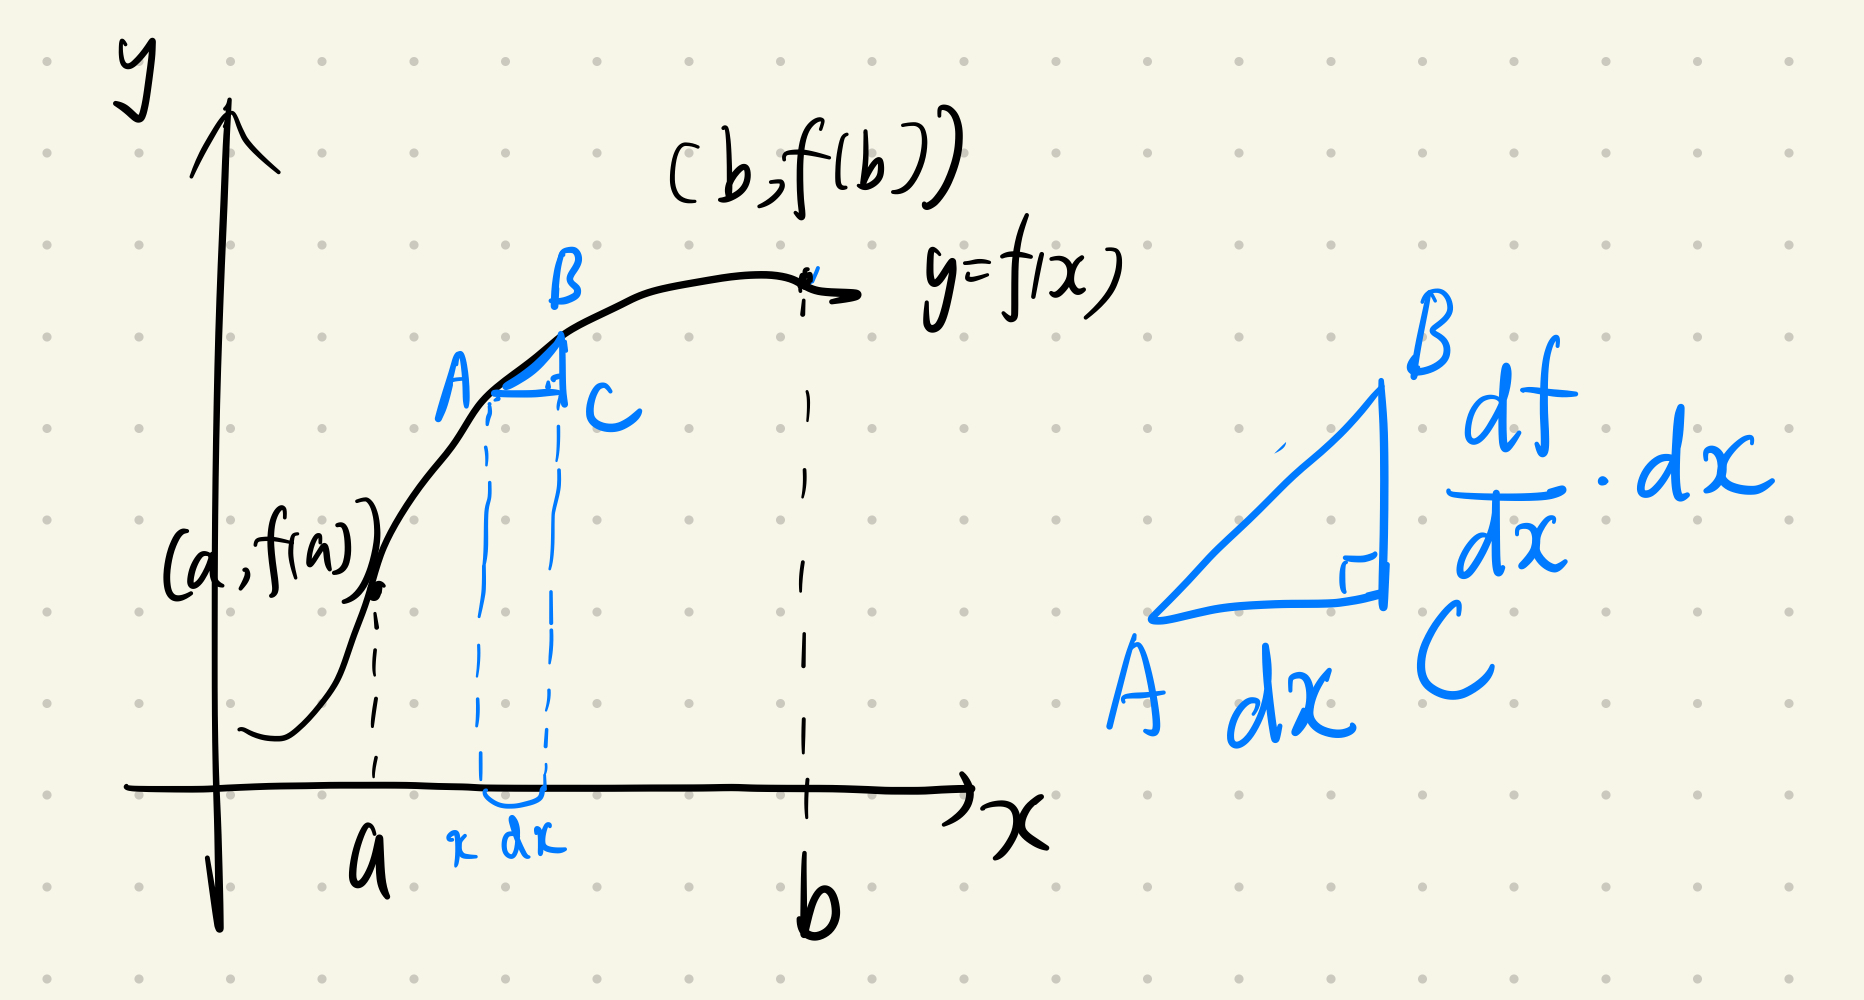
\includegraphics[width = 0.8\textwidth]{figures/chap 07/arc_length.png}
\end{figure}

As with previously where we broke up the area of interest into small strips of rectangles, here we break up the arc into small segments, shown as $\overline{AB}$ here.  As long as we can express $\overline{AB}$ as something shaped like $g(x)dx$, we can evaluate the arc length between $(a, f(a))$ and $(b, f(b))$ with the definite integral $\int_a^b g(x)~dx$.  

To find $g(x)$, we look at the right triangle $ABC$, magnified in the right panel of the graph above.  Given point $A$, point $B$ was constructed by taking an increment in $x$-coordinate by the differential $dx$, so we have $\overline{AC} = dx$.  The segment $\overline{BC}$ would then be the change in $f$ after the $x$-coordinate increment, which is the differential $df$ and can be alternatively written as $\frac{df}{dx}\cdot dx$.  Then, from the Pythagorean theorem:
\[\overline{AB} = \sqrt{\overline{AC}^2+\overline{BC}^2} = \sqrt{(dx)^2 + \Big(\frac{df}{dx}dx\Big)^2} = \sqrt{1 + \Big(\frac{df}{dx}\Big)^2}dx\]
Therefore, we have $g(x) = \sqrt{1 + \Big(\frac{df}{dx}\Big)^2}$, and the arc length is
\[S = \int_a^b \sqrt{1 + \Big(\frac{df}{dx}\Big)^2}dx\]
Let us try to evaluate a few arc lengths with our new formula:
\begin{eg}[]{eg: arc_length}
    Find the following arc lengths
    \begin{enumerate}[a)]
        \item The arc length of $y = \sqrt{1-x^2}$ between $x = -1$ and $x = 1$
        \item The arc length of $y = x^{3/2}$ between $x = 0$ and $x = 4$
        \item The arc length of $y = \ln(\sec x)$ between $x = \pi/6$ and $x = \pi/4$
    \end{enumerate}
\end{eg}

\begin{egsol}[]{egsol: arc_length}
    Find the following arc lengths
    \begin{enumerate}[a)]
        \item It is clear the $y = \sqrt{1-x^2}$ is the upper half of a circle centered at the origin with radius $1$, so our arc length should be half the circumference of a circle of radius $1$, which is $\pi$.  We can verify this by noting $\frac{dy}{dx} = -\frac{x}{\sqrt{1-x^2}}$, so the arc length should be
        \begin{align*}
            S &= \int_{-1}^1 \sqrt{1+\Big(\frac{dy}{dx}\Big)^2}~dx\\
            &= \int_{-1}^1 \sqrt{1+\Big(-\frac{x}{\sqrt{1-x^2}}\Big)^2}~dx\\
            &= \int_{-1}^1 \frac{1}{\sqrt{1-x^2}}~dx\\
            &= \arcsin x\Big]_{-1}^1 = \frac{\pi}{2} - \Big(-\frac{\pi}{2}\Big) = \pi
        \end{align*}
        where is identical to what we have predicted.
        \item Since $\frac{dy}{dx} = \frac{d x^{3/2}}{dx} = \frac{3}{2} \sqrt{x}$, the arc length can be evaluated by
        \begin{align*}
            S &= \int_0^4\sqrt{1+\Big(\frac{dy}{dx}\Big)^2}~dx\\
            &= \int_0^4\sqrt{1+\big(\frac{3}{2}\sqrt{x}\big)^2}~dx\\
            &= \int_0^4\sqrt{1+\frac{9}{4}x}~dx
        \end{align*}
        Now let $u = 1+\frac{9}{4}x$, so that $du = \frac{9}{4}dx$.  In addition, for the integration limits, when $x = 4$, $u = 10$; when $x = 0$, $u = 1$.  Therefore we have
        \begin{align*}
            S &= \int_0^4\sqrt{1+\frac{9}{4}x}~dx\\
            &=\frac{4}{9} \int_0^4\sqrt{1+\frac{9}{4}x}~\Big(\frac{9}{4}dx\Big)\\
            &=\frac{4}{9}  \int_1^10\sqrt{u}~du\\
            &= \frac{4}{9}\cdot \frac{2}{3}u^{3/2}\Big]_1^10 = \frac{8}{27}(10\sqrt{10}-1)
        \end{align*}
        \item Since $\frac{dy}{dx} = \frac{d \ln(\sec x)}{dx} = \tan x$, the arc length can be evaluated by
        \begin{align*}
            S &= \int_{\pi/6}^{\pi/4}\sqrt{1+\Big(\frac{dy}{dx}\Big)^2}~dx\\
            &= \int_{\pi/6}^{\pi/4}\sqrt{1+\tan^2 x}~dx\\
            &= \int_{\pi/6}^{\pi/4} \sec x~dx\\
            &= \ln|\sec x + \tan x|\big]_{\pi/6}^{\pi/4}\\
            &= \ln|\sqrt{2} + 1| - \ln|\frac{2}{\sqrt{3}}+\frac{1}{\sqrt{3}}| = \ln \frac{\sqrt{2}+1}{\sqrt{3}}
        \end{align*}
    \end{enumerate}
\end{egsol}

\begin{ex}[]{ex: arc_length}
    Find the arc length of $y = x^2$ between $x = 0$ and $x = 1/2$
\end{ex}

\begin{exsol}[]{exsol: arc_length}
    Since $\frac{dy}{dx} = \frac{dx^2}{dx} = 2x$, the arc length can be evaluated by
    \[S = \int_0^{1/2} \sqrt{1+\Big(\frac{dy}{dx}\Big)^2}~dx = \int_0^{1/2} \sqrt{1+(2x)^2}~dx\]
    To eliminate the square root, we let $2x = \tan \theta$, so that $dx = \frac{1}{2}\sec^2 \theta d \theta$.  For the limits of integration, when $x = 1/2$, $\theta = \arctan 1 = \frac{\pi}{4}$; when $x = 0$, $\theta = \arctan 0 = 0$.  Therefore we have
    \[S = \int_0^{1/2} \sqrt{1+(2x)^2}~dx = \int_0^{\pi/4} \sqrt{1+\tan^2\theta}~\frac{1}{2}\sec^2\theta d\theta= \frac{1}{2} \int_0^{\pi/4} \sec^3\theta d\theta\]
    To evaluate $\int_0^{\pi/4} \sec^3\theta d\theta$, we will need to use integration by parts where $u = \sec \theta, dv/d\theta = \sec^2 \theta$, so that $du/dx = \sec\theta \tan\theta, v = \tan \theta$:
    \begin{align*}
        \int_0^{\pi/4} \sec^3\theta d\theta &= \int_0^{\pi/4} \sec \theta \cdot \sec^2 \theta~d\theta\\
        &= \sec \theta \tan \theta\big]_0^{\pi/4} - \int_0^{\pi/4} \sec\theta \tan\theta \cdot \tan\theta d\theta\\
        &= \sec \theta \tan \theta\big]_0^{\pi/4} - \int_0^{\pi/4} \sec\theta \tan^2\theta d\theta\\
        &= \sec \theta \tan \theta\big]_0^{\pi/4} - \int_0^{\pi/4} \sec\theta (\sec^2\theta -1) d\theta\\
        &= \sec \theta \tan \theta\big]_0^{\pi/4} - \int_0^{\pi/4} \sec^3\theta d\theta + \int_0^{\pi/4} \sec\theta~d\theta\\
        &= \sec \theta \tan \theta\big]_0^{\pi/4} + \ln|\sec\theta + \tan\theta|\big]_0^{\pi/4} - \int_0^{\pi/4} \sec^3\theta d\theta\\
    \end{align*}
    Now both sides of the equation has the definite integral of $\int_0^{\pi/4}\sec^3\theta~d\theta$, so we aggregate them to the left:
    \begin{align*}
        &2\int_0^{\pi/4}\sec^3\theta~d\theta\\
        = &\Big(\sec\frac{\pi}{4}\tan\frac{\pi}{4}-\sec 0 \tan 0\Big) + \Big(\ln|\sec\frac{\pi}{4}+\tan\frac{\pi}{4}|-\ln|\sec 0 + \tan 0|\Big)\\
        = & (\sqrt{2} -0)+ (\ln|\sqrt{2}+1|-\ln|1|) = \sqrt{2}+\ln(\sqrt{2}+1)
    \end{align*}
    Therefore, we have
    \[ S= \frac{1}{2}\int_0^{\pi/4}\sec^3\theta~d\theta = \frac{1}{4} \cdot 2\int_0^{\pi/4}\sec^3\theta~d\theta = \frac{1}{4}[\sqrt{2}+\ln(\sqrt{2}+1)]\]
\end{exsol}

\section{Volume and surface area for solids of revolution}

In the previous section we've seen that definite integrals can help us evaluate the area under the curve, area between two curves, and the arc length of a curve.  We arrived at these definite integrals by slicing the area or arc length into pieces that can be expressed with $g(x)dx$, and then integrating them back to obtain the area or arc length of interest.  In this section, we will show that definite integrals can also help us evaluate the volume and surface area for solids of revolution, which are solids that has at least one axis of rotational symmetry, eg. a ball, an ellipsoid or a cone. 

Suppose a solid of revolution can be created by taking a curve $y = f(x)$ from $x = a$ to $x = b$ and rotating it about the $x$-axis.  For example, in the following graph, we have a clay pot-shaped solid that is rotationally symmetric along the $x$-axis.  Then, analogous to our previous approach, to evaluate the volume of the solid, we can slice the solid along the $x$-axis to get a series of thin disks.  If the volume of these disks can be expressed in the form of $g(x)dx$, then we can integrate $g(x)$ along the $x$-axis from $x=a$ to $x=b$ to get our desired volume.  

\begin{figure}[ht]
    \centering
    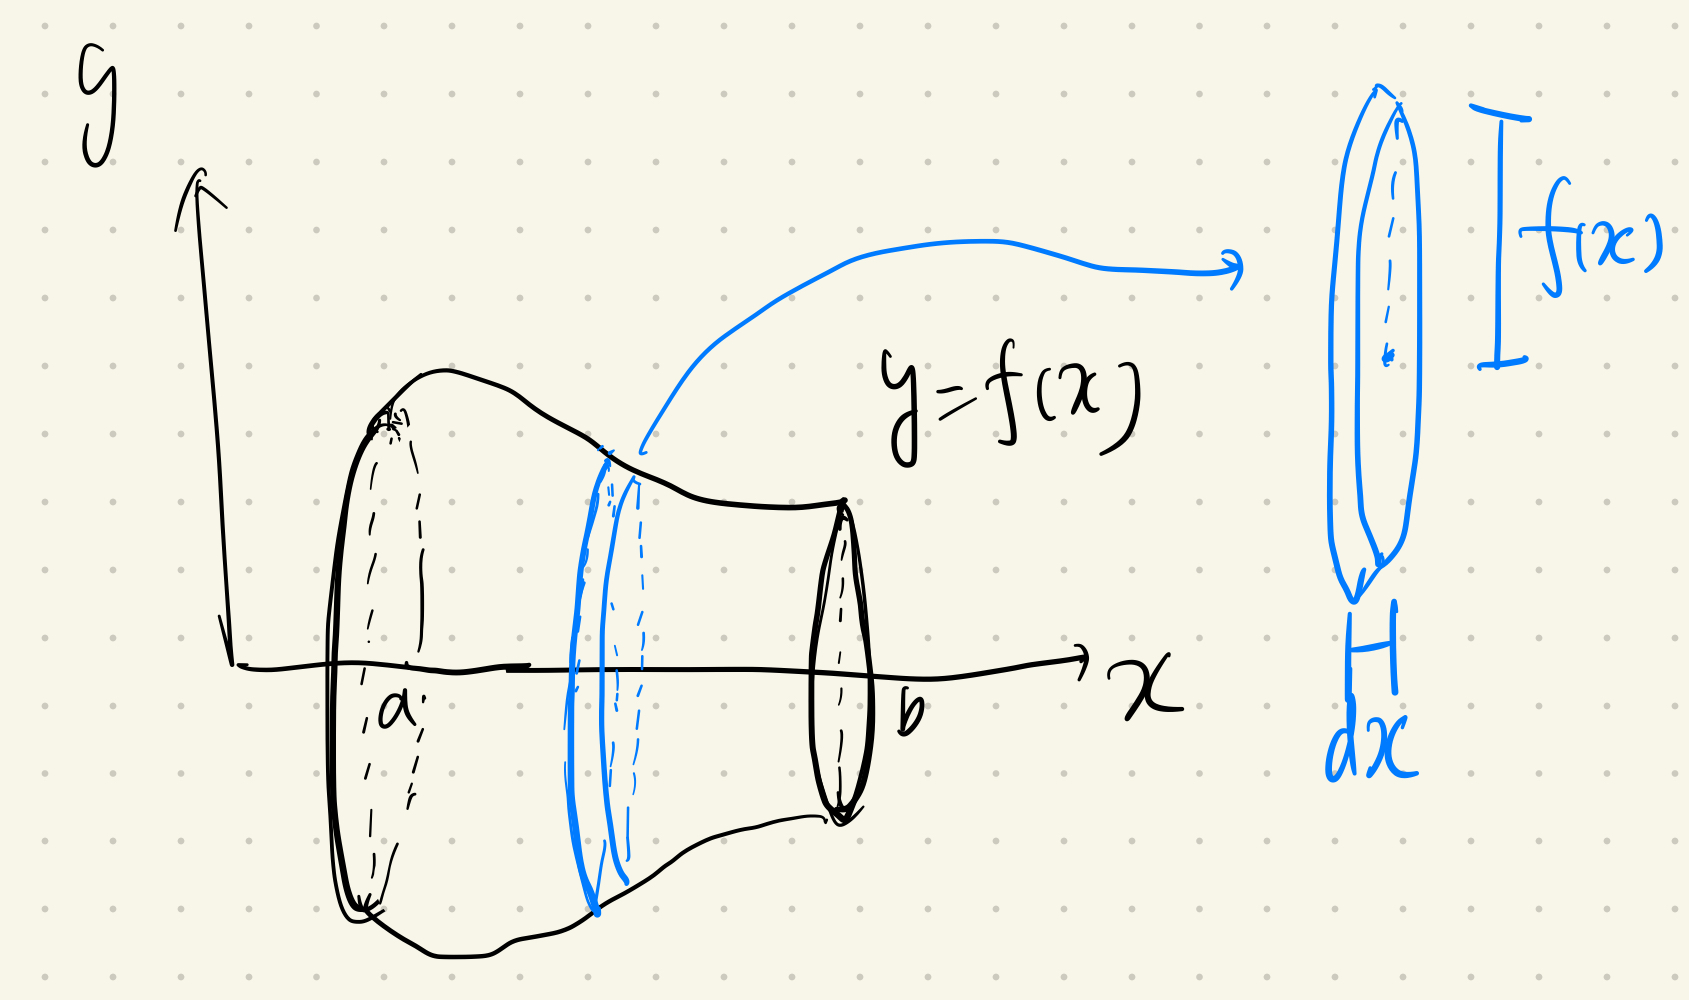
\includegraphics[width = 0.6\textwidth]{figures/chap 07/revolution_vol.png}
\end{figure}

The right panel of the graph above shows one slice of the thin disk.  As the disk gets thinner and thinner, it is approaching the shape of the cylinder.  Therefore, to evaluate the volume of the disk, we need to know the area of its base and its width.  For the height, since we are slicing along the $x$-axis, the width of the disk would be the differential $dx$.  For the area of its base, since this is a rotational solid, the section of each disk would a circle, with its radius as $f(x)$ since we are rotating $y = f(x)$ around the $x$-axis.  Therefore, the area of the base should be $\pi (f(x))^2$, and the volume of the disk is then $\pi (f(x))^2 dx$.  At last, the volume for the solid of revolution would be
\[V = \int_a^b \pi (f(x))^2~dx\]

\begin{figure}[ht]
    \centering
    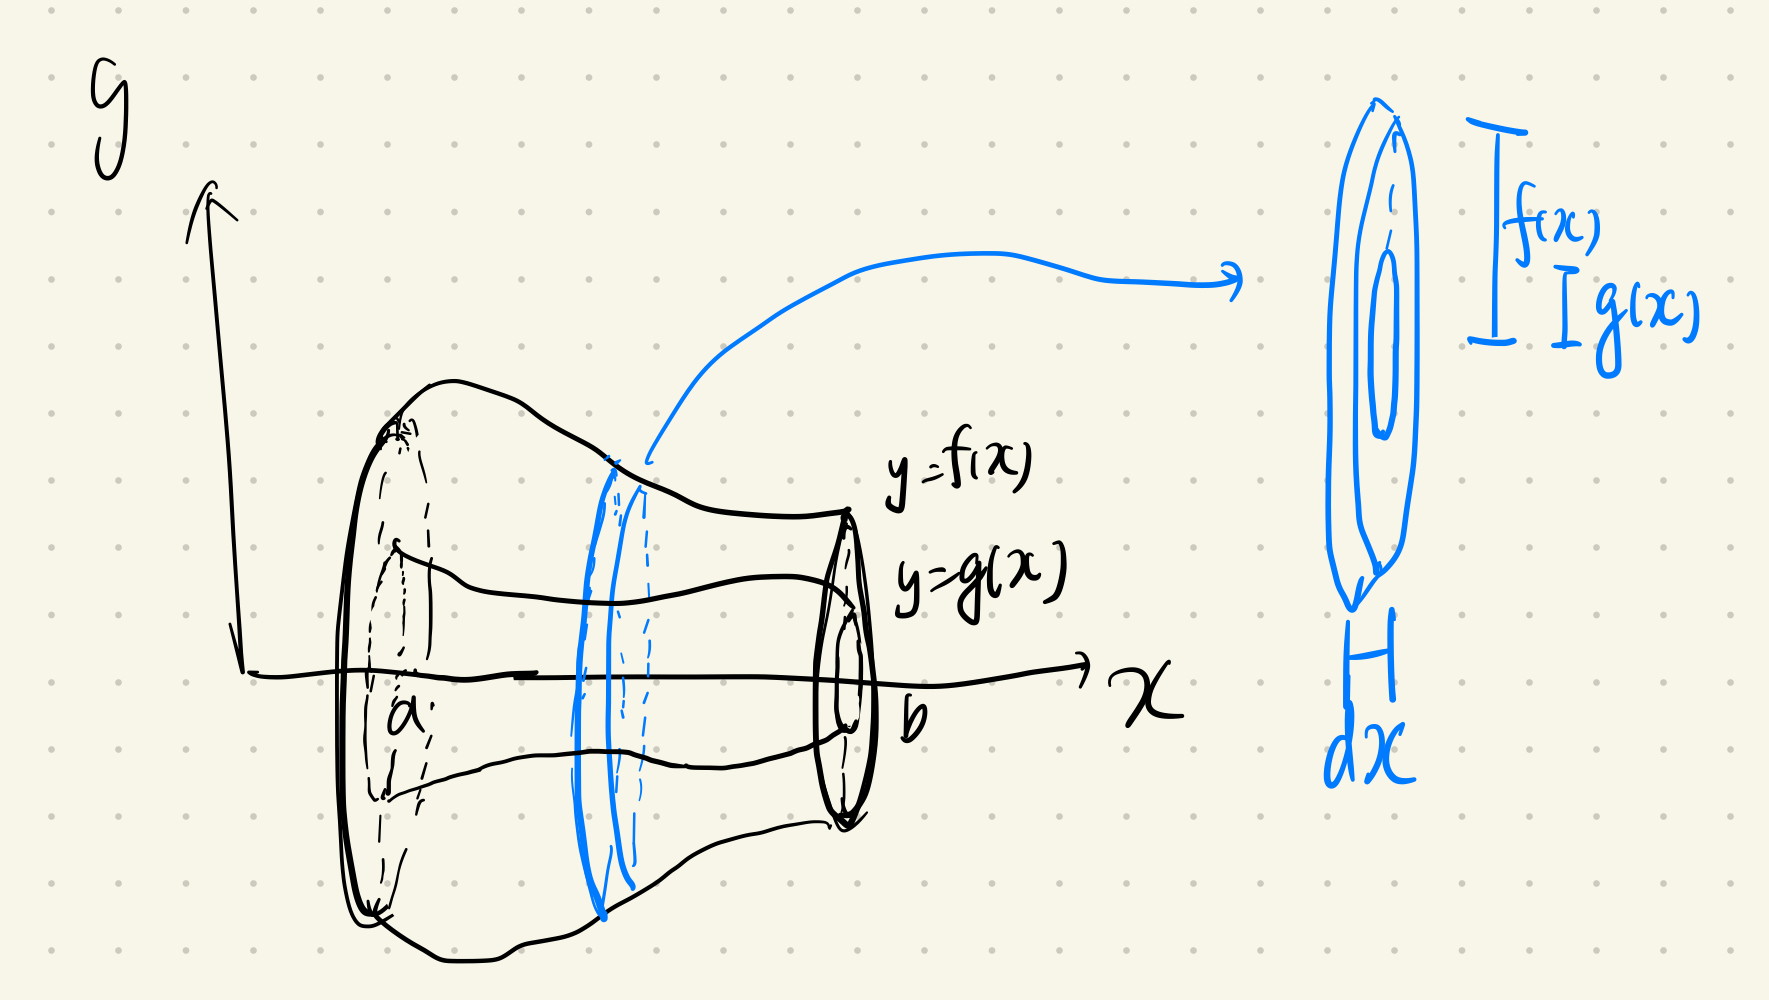
\includegraphics[width = 0.6\textwidth]{figures/chap 07/revolution_vol_ring.png}
\end{figure}

In the case where the solid revolution is formed by rotating the area between two curves along the $x$-axis, such as the graph above where the area between $y=f(x)$ and $y=g(x)$ are rotated, then volume of the thin disks would be instead $\pi [(f(x))^2-(g(x))^2] dx$ since we have to subtract the volume of the inner cylinder from the outer cylinder.  Therefore, the volume for the hallow solid of revolution would be 
\[V = \int_a^b \pi [(f(x))^2-(g(x))^2]~dx\]

Here our method slices the solid of revolution into disks or rings, depending on if the solid is hallow inside.  Therefore, this method is sometimes termed as the \textit{method of disks} or \textit{method of rings}.  We now show how they work with some examples:

\begin{eg}[]{eg: rev_solid_vol_ring}
    Verify the volume of the following solids using the method of disks
    \begin{enumerate}[a)]
        \item A ball of radius $r$ has volume $\frac{4}{3}\pi r^3$.
        \item A cone of height $h$ and radius of base $r$ has volume $\frac{1}{3}\pi r^2 h$.
    \end{enumerate}
\end{eg}

\begin{egsol}[]{egsol: rev_solid_vol_ring}
    \begin{enumerate}[a)]
        \item If we put a semi-circle of radius $r$ on the $x$-axis and rotate it about the axis, then we would get a ball or radius $r$ as the solid of revolution.  Therefore, as shown in the graph below, we can let $y = f(x) = \sqrt{r^2-x^2}$, which represents a semi-circle of radius $r$ with center at the origin, and evaluate the volume for the solid of revolution from $x = -r$ to $x = r$, which yields
        \begin{center}
            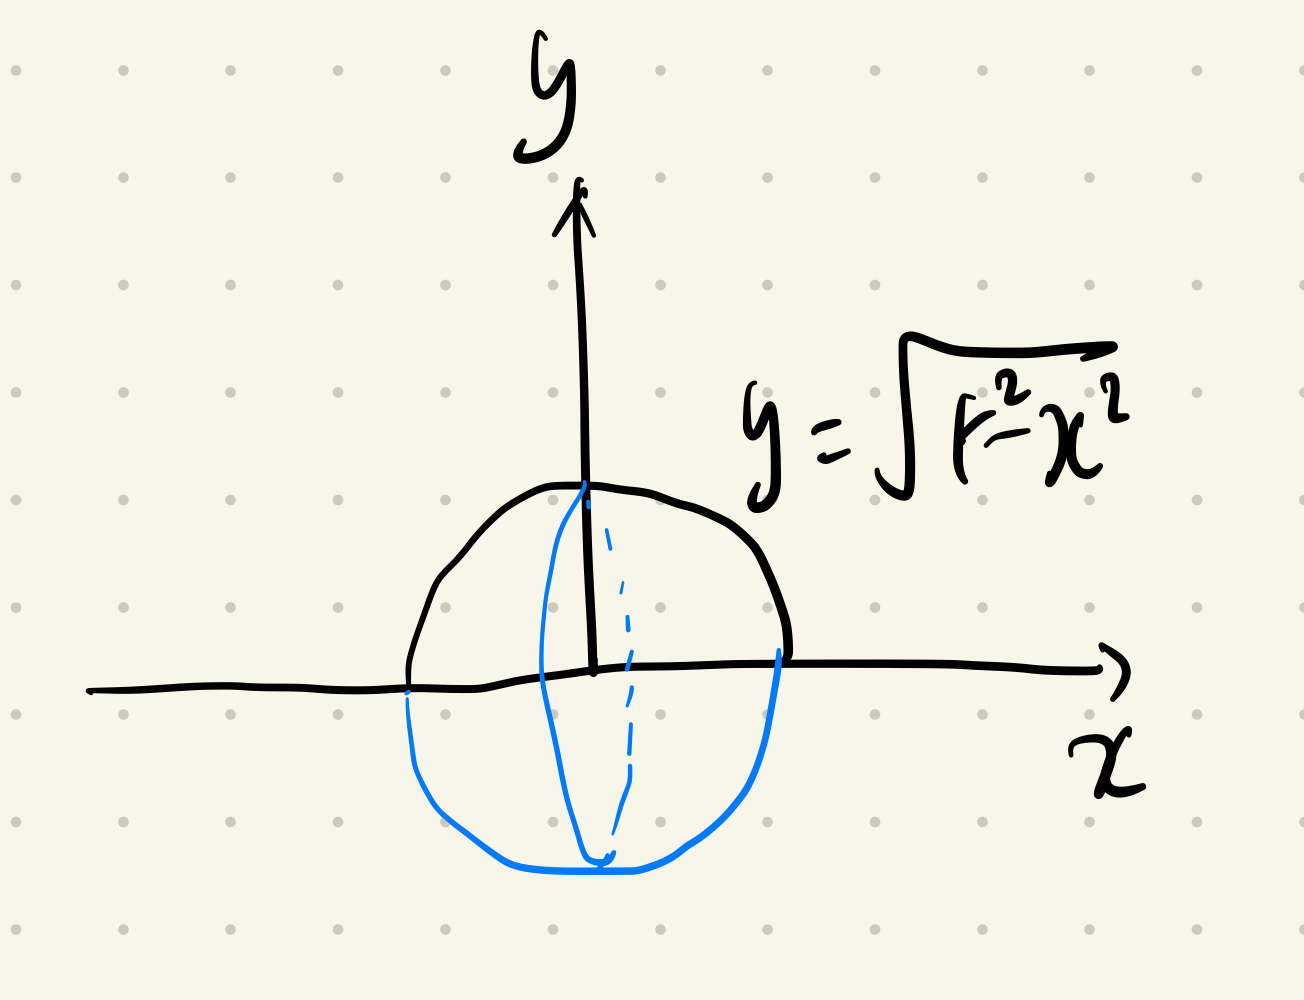
\includegraphics[width = 0.3\textwidth]{figures/chap 07/rev_solid_ball.png}
        \end{center}
        \begin{align*}
            V &= \int_{-r}^r \pi (\sqrt{r^2-x^2})^2~dx\\
            &= \int_{-r}^r (\pi r^2 - \pi x^2) ~dx\\
            &= \pi r^2 x - \frac{1}{3} \pi x^3\big]{-r}^r\\
            &= (\pi r^2 \cdot r - \frac{1}{3} \pi r^3) - ((\pi r^2 \cdot (-r) - \frac{1}{3} \pi (-r)^3))\\
            &= \big(1-\frac{1}{3} + 1 - \frac{1}{3}\big)r^3 = \frac{4}{3}\pi r^3
        \end{align*}
        \item As shown in the following graph, if we rotate a right angle triangle with base $h$ and height $r$ about the $x$-axis, we would get a cone described by the problem.  The hypotenuse of the triangle would have a slope of $r/h$, so its equation would be $y = (r/h)x$.  We can thus evaluate the volume for the solid of revolution from $x = 0$ to $x = h$ for $y = (r/h) x$, which yields
        \begin{center}
            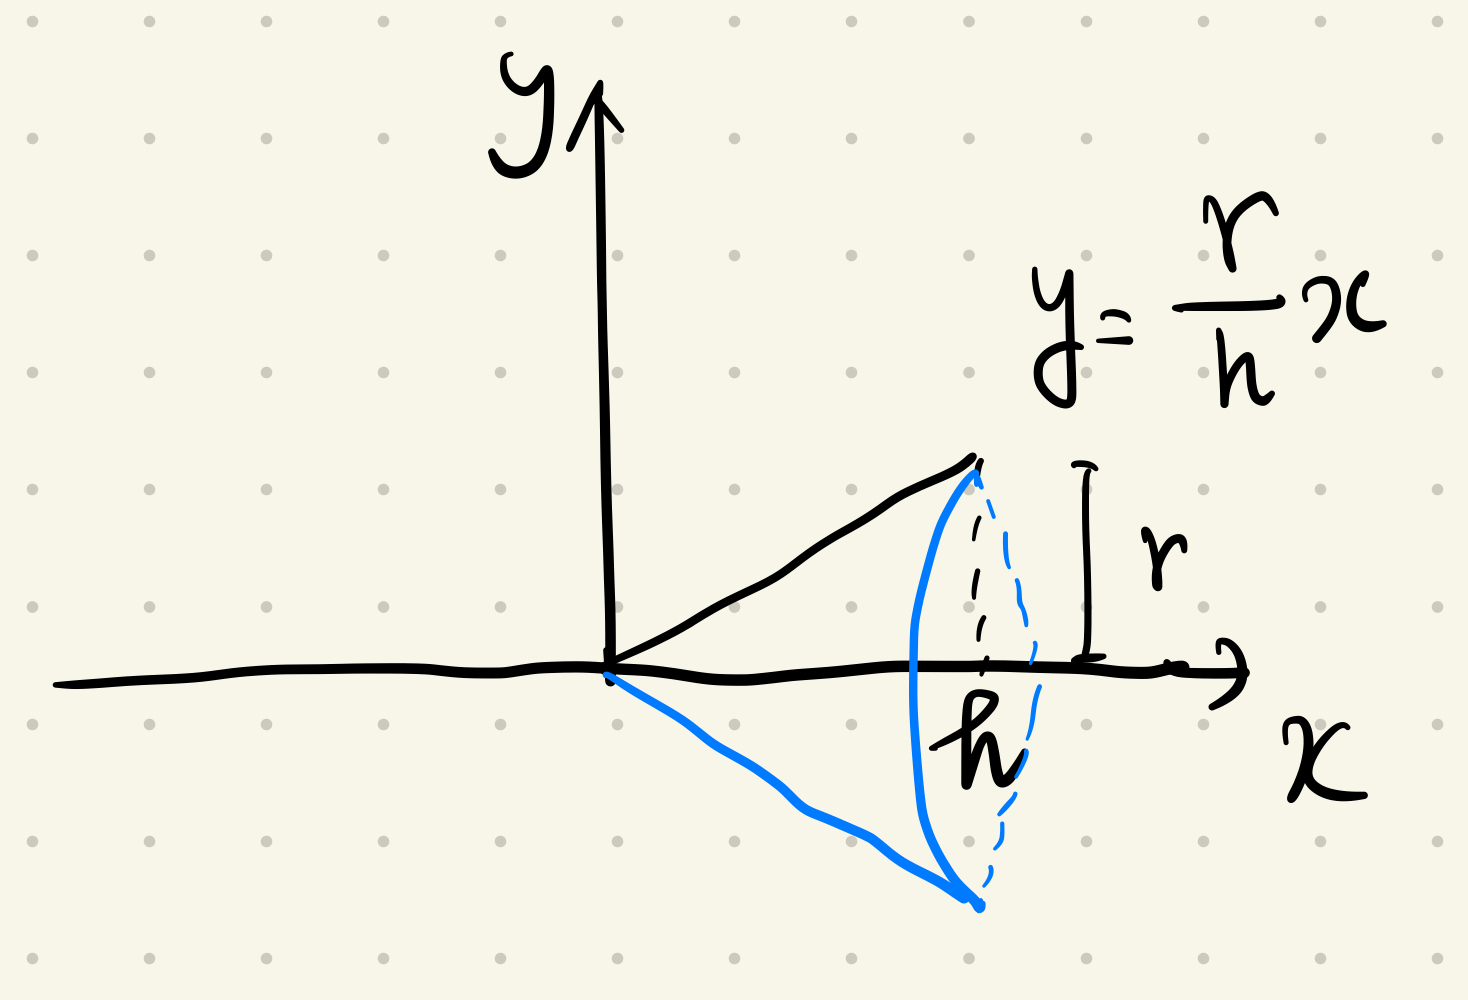
\includegraphics[width = 0.3\textwidth]{figures/chap 07/rev_solid_cone.png}
        \end{center}
        \begin{align*}
            V &= \int_0^h \pi \big(\frac{r}{h}x)^2~dx\\
            &= \int_0^h \pi \frac{r^2}{h^2} x^2~dx\\
            &= \pi \frac{r^2}{h^2} \cdot \frac{1}{3}x^3 \Big]_0^h\\
            &= \pi \frac{r^2}{h^2} \cdot \frac{1}{3}h^3 = \frac{1}{3} \pi r^2 h
        \end{align*}
    \end{enumerate}

\end{egsol}